\documentclass{article}

\title{Geonomics: A Python package for building agent-based, spatially explicit, and arbitrarily complex landscape-genomic simulations}
\author{Drew Hart}
%\date{January 18, 2019}

%%%%%%%%%%%%%%%%%%%%%%%%%%%%%%%%%%%%%%%%%%%%%%%%%%%%%%%%%%%%%%
% TODO:

% 1] update images
        % bottleneck: perhaps add a graph of the expected persistence times under bottleneck vs non-bottleneck, compared to observed times
        % stepstone: fix the legend on the Fst by island distance plot
                    %get rid of the mean pop-size plot
                    % fix legend on third plot
                    % run for ~ 30K timesteps, to see if Fst vals actually approach the expectation once most alleles should have fixed in the pops if they were fully isolated
        % divergence: run again and see if results are still so divergent from expectations (and if so probe the reason)
                    % axis fontsize 12, and get rid of titles
        % cline: axis fontsize 12, and get rid of titles
        % sweep: run again, to make sure axis and titles and stuff are correct
                 % make mean fitness a separate plot
        % PCA: get rid of titles, fix axis text size
        % two-trait: fix titles, axis text, etc
                 % otherwise leave as is, to discuss during lab mtg?
        % yosemite example: maybe make the plots manually, so that there's much less space between them all

% 2] improve captions

% 3] finish runtime analysis and add that section

% 4] add conclusion

%%%%%%%%%%%%%%%%%%%%%%%%%%%%%%%%%%%%%%%%%%%%%%%%%%%%%%%%%%%%%%

% load packages
\usepackage{graphicx} % to include graphics
\usepackage{url}      % to include URLs
\usepackage{fullpage} % use 1-inch margins
\usepackage{amsmath}  % for creating equations
\usepackage[font=footnotesize, labelfont=bf]{caption}  % create figure captions
\usepackage{hyperref} % for creating hyperlinks, both within-text and for URLs
\usepackage[all]{hypcap} %for going to the top of an image when a figure reference is clicked
\usepackage{cite}     % for bibtex citations
\usepackage{float}    % for controlling placement of floats (i.e. figures, etc.)

% create typewriter environment
\newenvironment{allintypewriter}{\ttfamily}{\par}


% define a 'centerfloat' by stealing code from
% https://tex.stackexchange.com/questions/16582/center-figure-that-is-wider-than-textwidth,
% which stole the code from the memoir class;
% this will horizontally center figures for which I call it
\makeatletter
\newcommand*{\centerfloat}{%
    \parindent \z@
    \leftskip \z@ \@plus 1fil \@minus \textwidth
    \rightskip\leftskip
    \parfillskip \z@skip}
\makeatother


\begin{document}

\maketitle


\section{Abstract}
{\LARGE TO BE COMPLETED}


\section{Intro/Background}
There is ever-growing interest in understanding and even predicting
the genomic evolution of complex study systems on complex and changing landscapes.
These systems might include one or multiple populations or species that are not
at demographic equilibrium. These species might inhabit complex, multivariate, and even changing landscapes.
And they may be undergoing neutral evolution as well as natural selection,
often on multiple traits of variable genetic architecture.
The field of landscape genomics studies the ways in which ecological and evolutionary
processes playing out on real landscapes
generate geographical patterns of genomic diversity,
Landscape genomics studies frequently feature analysis of data collected
from study systems of such
genomic and geospatial complexity~\cite{lind,mastretta-yanes,harris,crossley}. 
Study of such systems is crucial for developing
evolutionary and ecological theory~\cite{pelletier,barrett},
improving our knowledge of the past states and present functionality of ecosystems~\cite{mastretta-yanes},
anticipating ecological futures in the Anthropocene~\cite{bay},
and informing conservation and management~\cite{mastretta-yanes,crossley,lind}.

The complex genomics of such systems are beyond the reach of analytical
population genetics, and their spatial complexity and multifaceted evolutionary
dynamics make them intractable for coalescent simulation.
This hinders not only our understanding of many empirical systems and our ability to
unambiguously interpret analytical results, but also our
ability to predict those systems' dynamics, and thus to manage them appropriately.
Thus, as is increasingly the case in many fields, forward-time simulation is a 
crucial tool for dissecting the evolutionary dynamics of complex study systems in landscape genomics.
However, the current suite of forward-time genomic simulators, however numerous, is still of limited use for such work.
Most available software is limited, either genomically or geospatially, in the complexity it can model.
Many programs can model systems of considerable genomic complexity
(e.g.\ simuPOP~\cite{peng}, NEMO~\cite{guillaume} and QuantiNemo~\cite{neuenschwander}),
yet incorporate only rudimentary spatial components or none at all.
Other programs are designed specifically for landscape-genetic simulations
(e.g. CDPOP~\cite{landguth}, CDmetaPOP~\cite{landguth2}, SimAdapt~\cite{rebaudo}),
but are limited in their genomic complexity.
For instance, many programs are incapable of modeling simultaneous selection on numerous multigenic traits.
To our knowledge, SLiM~\cite{messer,haller}is the only package currently capable of simulating scenarios
that are both as genomically and as geospatially complex as those for which Geonomics is designed~\cite{popgen_models}.
(Indeed, the generalizability and complexity of which SLiM is capable far exceeds that of Geonomics.)

We developed Geonomics to provide a scriptable framework for building
complex landscape-genomic simulations with minimal effort.
Geonomics models are parameterized by way of an informatively annotated parameters file
that provides the user a straightforward means of building models of arbitrary complexity, yet offers
reasonable default settings and/or `off switches' for model components
that are not the focus the user's interest.
Models consist of a landscape, composed of one or more environmental layers,
and one or more species, each described by a variety of life-history parameters
and a genomic architecture of arbitrary complexity that may be mapped onto
one or more traits under seleciton.
Landscape layers may be used to control various aspects of a species' functionality,
including carrying capacity, movement and offspring dispersal, and natural selection).
Landscape layers and species can undergo one or more environmental and demographic change events
over the course of a model run.
At each timestep, a species undergoes movement (in continuous space),
mating (using realistic genomics and generating additive phenotypes),
mortality (by both  density-dependence and selection),
and change events (at the timesteps for which they are scheduled).


The complex landscape-genomic models for which Geonomics is designed would require a considerable amount
of work to script in SLiM's Eidos framework (see examples of spatialized selection in SLiM 2's recipe book;
e.g.\ section 14.11, page 288;~\cite{slim_manual}), but can be built in Geonomics
with an edited parameters file and as little as three lines of code.
For example, a Geonomics user could build a model of evolution with natural selection
on multiple multigenic traits, on a multivariate landscape undergoing spatially inhomogeneous
environmental change for certain landscape layers, for a species moving realistically across that landscape,
and then run this model an arbitrary number of times, collecting data heterochronously during each
run --- all of this by doing nothing more than templating a parameters file, making alterations,
loading the file, and running the resulting model object.

What's more, Geonomics is written and run entirely in Python, a broad-purpose and popular
programming language that is already familiar to most researchers with exposure to bioinformatics.
This of course makes Geonomics considerably slower than its brethren that are
written in compiled languages such as C++ (e.g. SLiM). 
But within the range of reasonable parameter values (see section on runtime analysis, below), 
we do not expect runtime to be a major constraint for the sorts of models
for which Geonomics was designed.
And what Geonomics sacrifices in performance, it gains in flexibility, extensibility, and accessibility.
The basic user needn't even know how to write full Python scripts;
users can build their own models by recycling and tweaking
a minimal amount of code (available within the documentation and at the Geonomics homepage).
However, advanced users wishing to code their own extensions or customizations
have broad opportunity to do so,
because Geonomics is a Python package that seamlessly integrates into the universe of Python functionality.


\section{Model description}

\subsection{Components}
A Geonomics model consists of two core components: the species and the landscape.

\subsubsection{Species}
A species consists of an arbitrary number of individuals, which do not belong to
discrete populations but instead are distributed in continuous space upon the landscape.
A species is described by a wide variety of demographic and life-history parameters
that determine its behavior in the model (e.g.\ intrinsic growth rate, mate-search radius,
mean number of offspring per mating event, reproductive age and maximum age;
for a detailed discussion and these and all other model parameters, see the documentation).
Each species can also undergo any number of arbitrarily complex demographic changes during
each model run, including both population-size changes
(which can be exponential, cyclical, stochastic, or custom-defined)
and changes to demographic and life-history parameters.

Each individual in a species is described by an x,y location, a sex, an age (or stage),
a genome (optionally), and a phenotype for any traits assigned to the species.
(It is worth noting that species are collected into objects called communities,
which for most models will consist only of a single species,
but which provides a framework for the advanced user 
to code inter-species interactions for multi-species models;
this is a functionality that we hope to build into future versions of the software.)

Each individual has a diploid genome consisting of $L$ diallelic loci.
These loci can be treated as representing either a contiguous haplotype block
or a set of discrete markers, depending on the map of recombination rates assigned to the genome.
(For simplicity's sake, we refer to these loci herein, and in the software generally, as `the genome'.)
Genomes are initially assigned based on a species' genomic architecture---an object containing
parameters describing all simulated loci.
These parameters include the starting allele frequencies and dominance values for all loci,
the inter-locus recombination rates across the genome.
Separate chromosomes can be modeled by providing a list of chromosome lengths,
between which the recombination rate is set to 0.5, ensuring independent assortment.

A genomic architecture can also stipulate any number of traits for a species. Traits can be mono- or multigenic, and are quantitative and continuously valued.
Each trait is defined by a set of loci that underpin it, the effect sizes of those loci,
and a selection coefficient (which can be heterogeneous or homogeneous in both space and time).
Mutations, which are of three types: neutral; deleterious, which universally decrease an individual's fitness); 
and trait-affecting, which influence an individual's phenotype, with the resulting fitness effect
determined by the individual's local environment.
All three mutation types are controlled by type-specific mutation rates 
(additional parameters within the genomic architecture, any or all of which can be set to zero).
(To simulate complex, specific genomic architectures, users can provide a
CSV-formatted file defining the architecture locus by locus.
For details, see the documentation.)

\subsubsection{Landscape}
Aside from the species, the other core component in a Geonomics model is the landscape.
A landscape is a stack of an arbitrary number of layers (i.e.\ environmental variables),
each represented by a raster of normalized values ($0 \leq value \leq 1$).
Each layer can be programmed to serve as the basis for any of a number of model components:
1.\ the raster of cell-wise carrying-capacities controlling the population density of a species;
2.\ the resistance surface controlling the realistic movemement of individuals and/or 
dispersal of offspring across the landscape;
3.\ the selective force acting on one or more traits  of one or more species.

Each layer of a landscape can be programmed to undergo any number of
arbitrarily complex environmental change events during each model run.
The changes they produce will in turn affect the simulation by way
of any species on the landscape for which that layer plays a role in its
population dynamics, movement, dispersal, or natural selection.
Each event is defined by the timesteps over which it unfolds, and either the terminal
raster of the event (with intermediate rasters being linearly interpolated) 
or a directory containing the stepwise time-series of rasters pertaining to the event.
The latter option makes it extremely easy to simulate evolution on real-world
rasters undergoing real, non-linear, spatially heterogeneous environmental change.


\subsection{Operations}
A Geonomics model can be run for any number of runs,
with each run creating its own separate subdirectory of output.
At the start of each run, the model is burned in.
This is accomplished by iterating timesteps without genomes and
natural selection until a series of statistical tests for temporal
and spatial stability in population size is passed.
These tests include a time-lagged t-test of mean population size;
an augmented Dickey-Fuller test of population size;
and a {\large STILL NEED TO ADD THE SPATIAL TEST}.
Then, if genomes are being used, each individual has its genome randomly drawn
according to the species' genomic architecture, such that the `main' phase
of each run begins without population structure.
The main phase of the run can run for any number of timesteps. 
Each timestep is composed of a series of four core operations,
some requisite, some optional (see Figure~\ref{fig:flow} for depictions):
\begin{enumerate}
  \item \textbf{movement} (optional);
  \item \textbf{mating} (requisite; include mate search, mate choice, offspring creationg, and offspring dispersal);
  \item \textbf{mortality} (due to the combination of density-dependence [requisite] and natural selection [optional]);
  \item \textbf{change events} (both environmental and demographic; optional);
\end{enumerate}

Each individual's age/stage increments at the beginning of each timestep, and data and statstics are saved at the end when necessary.

Movement takes place in continuous space, such that individuals are not arbitrarily restricted to grid cells.
Individuals' distances and directions are drawn separately, then composed into movement vectors.
Distances are Wald-distributed (and the distributional parameters, as with nearly all distributions
used in the model, can be set by the user within a Geonomics parameters file).
Directions can either be drawn from a uniform distribution on the unit circle, resulting in isotropic movement
(the default behavior); or they can be drawn from a `movement surface'.
A movement surface is an array of uni- or multimodal Von Mises distributions,
derived from a landscape layer that serves as a resistance surface.
On a unimodal surface, each cell is assigned a Von Mises distribution that has $\mu$
equal to the direction of the centerpoint of the highest-valued neighboring cell
(using an 8-cell neighborhood) and has $\kappa$ set by the parameters file.
On a multimodal surface, each cell's mixture distribution is a weighted sum of eight such
unimodal distributions, one for each cell in its neighborhood
(with weights equal to the neighboring cells' values divided by their sum). 
This is, to our knowledge, a novel approach to simulating movement.
It generates realistic, anisotropic movment across an environment of heterogenous habitat quality, while avoiding the use of time-consuming neighborhood-querying functions during model runtime.
(See Figure~\ref{fig:move_surf} for depictions.)

Mating pairs are chosen from among all eligible pairs of individuals within the species' mate-search radius.
Eligibility can be based on age and sex.
Pair decisions are a Bernoulli draw, with probability equal to the species' intrinsic birth rate.
For each mating pair a number of offspring is chosen from a Poisson distribution (with
$\lambda$ equal to the species' mean number of offspring), unless it is set to a fixed value by the user.
Each parent produces one gamete for each of its offspring, by recombination---at 
the inter-locus rates defined by the species' genomic architecture---and 
Mendelian segregation.
Offspring individuals are created and then dispersed to a new location
(where, as with movement, the directions of their dispersal vectors can be drawn either isotropically or
anisotropically, the latter using a `dispersal surface' that is structurally
identical to a movement surface).

Mating is followed by mortality.
Deaths are Bernoulli draws, using individual-wise death probabilities that are
a combination of the probabilities of death by density-dependence
(from a spatialized logistic-growth model)
and by natural selection (on any number of traits simultaneously). 
This is calculated as:
\begin{equation}
        P(d_{i}) = 1 - (1 - P(d_{x,y})) \prod_{p = 1}^{m}\omega_{i,p}
\label{eqxn:prob_death_i}
\end{equation}
where $P(d_{x,y})$ is individual $i$'s probability of death by density-dependence
and $\omega_{i,p}$ is individual $i$'s fitness for trait $p$
(and only factors in if natural selection is being used).
The probability of density-dependent death at location $x,y$ is calculated as:
\begin{equation}
\begin{split}
       P(d_{x,y}) = E[N_{d;x,y}]/N_{x,y} = \frac{E[N_{b;x,y}] - \frac{\mathrm{d}N_{x,y}}{\mathrm{d}t}}{N_{x,y}}
\label{eqxn:prob_death_xy}
\end{split}
\end{equation}
where $E[N_{d;x,y}]$ is the expected number of deaths at the individual's $x,y$ location on the landscape;
$N_{x,y}$ is the population density (expressed as individuals per cell-area) at the location;
$E[N_{b;x,y}$ is the expected number of births at the location;
and $\frac{\mathrm{d}N_{x,y}}{\mathrm{d}t}$ is the logistic population growth rate at the location.
Individual $i$'s fitness for trait $p$ is calculated as:
\begin{equation}
        \omega_{i,p}= 1 - \phi_{p;x,y} {( \mid e_{p;x,y} - z_{i;p} \mid )}^{\gamma_{p}}
\label{eqxn:fitness}
\end{equation}
where $\phi_{p;x,y}$ is the selection coefficient on trait $p$ at the
individual's location; $e_{p;x,y}$ is the environmental value
of the layer that serves as the selective force for trait $p$i,
$\gamma_{p}$ defines the curvature of the fitness function for trait $p$,
and $z_{i;p}$ is individual $i$'s phenotype for trait $p$.
And individual's phenotype is a result of the additive effects of that
individual's genotypes at all influencing loci---Geonomics does not model
epistasis---and is calculated as:
\begin{equation}
        z_{i;p} = g_{0} + \sum_{l = 0}^{n} \alpha_{p,l} g_{i,l}
\label{eqxn:phenotype}
\end{equation}
where $n$ is the number of loci, $\alpha$ is a locus' effect size, $g$ is the
individual's genotype, and $g_{0}$ is 0 for monogenic traits,
0.5 for polygenic traits. 

Environmental and demographic change events can be scheduled to occur over
any desired portion of the total time of a run.
Each event unfolds through a series of incremental changes, which occur at the
timesteps specified in the parameters file.
In similar fashion, statistics are calculated and data are collected
at timesteps for which they are parameterized. 

Geonomics is designed as an object-oriented scripting framework with both basic and advanced modes.
The basic mode simply requires users to call a first command to create a template
parameters file (which they must then edit as desired), a second command to create
a model object from that parameters file, and a third command
to then run the desired number of runs for that model.
The advanced mode allows users to write more detailed scripts that make modifications
to the components of their models, or to collect custom data from their model,
by calling custom functions before a model is run, between any timesteps,
or after a run is complete.
(This is what makes Geonomics so extensible---because it is a Python package,
users can call on the full spectrum of Python functionality to design custom code
that operates on their Geonomics objects.)

\subsection{Validation}
We have run a series of tests to statistically heuristically validate
Geonomics' full range of functionality.
All test results matched expectations based on
population-genetic and genomic theory.
(For details, see Supplements.)

\section{Applications}

\subsection{Isolation by distance and by environment}
Many real-world populations inhabit complex, heterogeneous landscapes.
Landscape heterogeneity can constrain movement, and thus gene flow, when
the probability of an individual moving across each area of a landscape
is conditional on that area's environment.
Ecologists commonly use resistance surfaces to describe such movement~\cite{mcrae}.
Geonomics allows a user to load resistance surface layers, then use them as the basis
for creating movement and/or dispersal surfaces produce realistic movememnt patterns
(see Figure~\ref{fig:move_surf}).
In a Geonomics model containing such a landscape, realistically simulated movement 
should generate a realistic pattern of isolation by distance (IBD): 
Pairwise genetic distances between individuals, populations, or landscape regions, 
should be positively correlated with pairwise geographic distances.

Landscape heterogeneity can also underlie processes that generate a pattern of isolation
by environment (IBE).
This is a pattern in which pairwise genetic distances between
individuals, populations, or regions correlate positively with pairwise environmental distances, independently of pairwise geographic distances.
Geonomics' implementation of natural selection allows the selective regime to vary
across the landscape (both in its optimal phenotype and its strength of selection).
This models a key process that should produce realistic patterns of IBE: Spatially divergent selection.

To test Geonomics' ability to generate patterns of both IBD and IBE,
we constructed a model of a single species (roughly XXXX individuals)
undergoing both neutral and selective evolution on a landscape of two layers.
The first layer, which serves as the movement surface and the carrying-capacity raster,
consists of a central, vertical barrier separating equal-area sides within which
movement is unconstrained. 
The second layer, which serves as the selection layer, consists of two environmental gradients of inverse directionality, one on each side of the first layer's barrier.
As data, we collected the species' full set of genomes both at the beginning of the model
(just after the burn-in) and after the model ran to completion (1000 timesteps).
We ran genetic Principal Components Analysis (PCA) on these two datasets.
From each PCA, we extracted the first three principal components (PCs),
scaled them to $0 \leq value\leq 1$, then used the resulting numbers
to assign red, green, and blue (RGB) values to each individual.
We used each individual's value for those three values to create a colored
scatterplot of the species both before and after evolution.
We paired these with plots of the species, colored by their phenotypes for the trait
under selection (using Geonomics' `model.plot\_phenotype()` method).
We then also calculated and plotted correlations of pairwise (Euclidean) geographic
and environmental distances with scaled pairwise genetic distances, and used
logistic regression (with a `cloglog' link) to assess patterns of IBD and IBE.

The results show a clear lack of spatial structure at the outset
(Figure~\ref{fig:IBD_IBE}, row 1), because genomes were randomly drawn and assigned,
so the population possessed no spatial structure.
Spatial structure develops over evolutionary time
(Figure~\ref{fig:IBD_IBE}, row 2, left) concordant with the development
of local adaptation (Figure~\ref{fig:IBD_IBE}, row 2, right).
At the end of the simulation, the species demonstrates a
significant signal of both IBD (Figure~\ref{fig:IBD_IBE}, row 3, left)
nd IBE (Figure~\ref{fig:IBD_IBE}, row 3, right).


\subsection{Simultaneous selection}
One of the powerful features of Geonomics is that it can simulate selection
on numerous traits simultaneously, with the selection layer for each trait
being separately specified. 
Thus, a species can experience multiple, distinct selective regimes simultaneously.
This will prove useful for many landscape simulations, given that many natural systems
are hypothesized to be locally adapted to multiple, divergent environmental gradients.

We simulated a scenario in which a population undergoes natural selection along two, orthogonally
aligned environmental gradients. Each gradient serves as the selective force ($s = 0.05$)
for a separate trait.
Each trait is composed of 10 distinct, unlinked loci, all with effect sizes of 0.1
(i.e.\ one tenth of the distance between the two opposite, optimal phenotypes).

Results show a clear signal of local adaptation to both gradients, as can be see in
maps of the final population colored according to their phenotypes for each of their
two traits~\ref{fig:sim_sel}.


\subsection{Polygenic adaptation to climate change in the Yosemite region}
Geonomics' full use-value is best demonstrated by walking through a complex, worked example.
In this section, we explain a complex evolutionary scenario, 
explain the steps we used to simulate it, then present the results.
(The source code for this example is available within the
\texttt{./example/yosemite} directory of the Geonomics package directory.)

There is growing interest in the evolutionary implications of climate change.
Much of this interest focuses on species that are locally adapted along an
environmental gradient that is expected to shift under climate change.
Climatic shifts can be spatially non-homogeneous, because many cooler,
higher-altitude regions are warming more quickly than warmer,
low-altitude regions, and are projected to continue doing
so~\cite{rangwala,mountain_research_initiative} (but, see~\cite{oyler}).
Of particular interest in these situations is the ability of species to adapt
to changing local conditions. Of the possible species responses to climate
change---the others being range shifts, plasticity, tolerance, and local
extinction---this is the response about which we know the least.

To show Geonomics' utility for studying such a system,
we simulate the evolutionary response to projected climate change
of a continuously distributed, locally adapted species:
the montane lizard \emph{Sceloporus graciosus} ("sagebrush lizard"),
in the Yosemite region of California (U.S.A.).

We began by preparing the raster layers to be used for the model's landscape.
These include a time-series of temperature rasters and a time-series of habitat-suitability rasters.
(Note that both in the preparation of our temperature
data and in the production of our SDM we use simplistic assumptions and minimal complexity,
because the purpose of this example is only to demonstrate the utility of our software.)
All data preparation was done using custom scripts (available in the supplements) in
the R statistical programming language~\cite{Rlang}.

The first set of layers consists of current mean annual temperature and its projections
through year 2100 (the latest available year).
For current temperature we use PRISM~\cite{daly} data: 30-year normals (1981-2010),
800-m resolution, PRISM v.14.1.
For future years, we use minimum and maximum annual temperature data at 5-year intervals (2015-2100)
and 6-km resolution, downloaded from \href{https://cal-adapt.org/help/faq/}{Cal-Adapt}.
This data consists of climate projections that were downscaled using the Localized Constructed Analogs, downscaling technique (LOCA;~\cite{pierce}).
The data are the minima and maxima observed across 32 LOCA-downscaled global climate models,
using a conservative representative concentration pathway (RCP 4.5).
We use this data to develop a time-series of future temperature layers at our 800-m current-temperature resolution,
according to the following algorithm:
\begin{enumerate}
        \item calculate the average of the minimum and maximum rasters for the first future year (2015);
        \item extract the values of those two rasters for the top-left cell;
        \item calculate the mean of those values;
        \item find all cells in the 800-m PRISM raster that fall within this cell;
        \item for each of those cells, add the difference between its current value and the average projected value to its current value;
        \item repeat steps 2. to 5. for all cells in this year's minimum and maximum rasters, gathering the resulting 800-m cells into a projected, 800-m raster;
        \item repeat steps 1. to 6. for all remaining years, gathering the resulting rasters into a projected climate-change time-series;
\end{enumerate}

The second set of layers consists of \emph{S. graciosus} habitat-suitability layers, which
we developed from a species distribution model (SDM) using a
binomial genearlized linear model (GLM) with a logit link.
Our SDM was constructed according to standard theory and practice~\cite{peterson}.
We downloaded all geotagged occurrences of \emph{S. graciosus} from \href{https://www.gbif.org}{GBIF}
(accessed 10:33 a.m. PST on March 5, 2019).
For presence data, we clipped those points to the area of California and Nevada,
and subsampled to remove multiple points within the same raster cells.
Per recommendation for regression-based SDMs, we generated pseudoabsence data by drawing random points
in the California-Nevada region, outside of cells where presences were observed~\cite{barbet-massin}.
We extracted the 30-year normals temperature data to these points, which we used as a predictor
variable of presence/pseudoabsence in our GLM.
We then projected that GLM onto the full current and future temperature rasters of our study region,
producing a time-series of predicted habitat suitability across our region
(where $0 \leq suitability \leq 1$).
(We did not threshold these rasters for a minimum suitability value.
We preferred to allow the product of these rasters and our species'
parameterized carrying-capacity constant to produce, in Geonomics, rasters of
continually decreasing carrying capacity that would, in turn,
produce a pattern of continually decreasing population density toward the species' range edges.)

With these rasters prepared, the construction of our Geonomics model was straightforward.
We generated a template Geonomics parameters file
(using \texttt{gnx.make\_parameters\_file(\ldots)}),
then edited it to match our study system.
We needed a parameters file that could parameterize: 2 `file'-type Layers
(i.e.\ layers red in from files; see the Geonomics documentation for details),
both of which would undergo landscape-change;
1 Species, with movement, a movement-surface, and genomes with 1 trait;
and data-collection.
The Geonomics command we ran to generate a template Geonomics parameters
file with those components was:

\begin{allintypewriter}
>>> gnx.make\_parameters\_file(filepath=`yosemite\_params.py',\\
                               layers=[\{`type': `file', `change': True\},\\
                                       \{`type': `file', `change': True\}],\\
                               species=[\{`movement': True, `movement\_surface': True,\\
                                          `genomes': True, `n\_traits': 1\}],\\
                               data=True)\\
\end{allintypewriter}

We edited the resulting file, setting the appropriate parameter values to indicate
the locations of our starting temperature and habitat-suitability rasters
and the locations of our directories of change rasters for
those layers. We set other life-history and demographic parameters to reasonable values,
based on current knowledge of \emph{S. graciosus} biology (see parameters file, in Supplements,
for full details).

Then, in a Python script (also in the Supplements), we used our parameters file to
create a Geonomics model object (using \texttt{model = gnx.make\_model(\ldots)}), then
ran that model. We used \texttt{model.walk(\ldots)} to run the burn-in,
run the main phase for 500 pre-climate change timesteps
(to develop a pattern of local adaptation),
then run the main phase for an additional 100 timesteps of climate change.
The \texttt{model.walk} function is what we refer to as Geonomics' `advanced' mode above;
as opposed to \texttt{model.run}, it allows the user to run the model for only a certain number
of timesteps, then pause it to call their own custom code.
In our case, we stopped the model at timesteps 500 (before climate change) and 600
(after climate change), each time plotting the landscape layers, the population,
and a neighborhood-meaned raster of the population's phenotypes (using a custom
function written in-script).

This produced the results visible in~\ref{fig:yosemite}.
The model generates a clear and realistic pattern of polygenic adaptation to
the elevation-based temperature gradient in the Yosemite region, and that
gradient of local adpatation exhibits a pronounced upslope shift in response to
the period of climate change. These results are visible both heuristically
(from the individuals' phenotypes plotted before and after climate change)
and analytically (from the neighborhood-meaned phenotype rasters plotted at the same timepoints).
Population size is roughly 34,000 before climate change, declining to roughly 27,000
at the end of the simulation.


\section{Discussion}

\large{~2 paragraphs summarizing key points and outcomes}
- we have created a new piece of software that makes complex landscape-genomic modeling
simpler and more accessible
- we think it will be useful for many modeling purposes
- all of our examples (as well as our validations tests) give us a high level of confidence
in Geonomics' ability to accurately model the sorts of systems for which it is designed

\subsection{Runtime and memory}
As mentioned above, Geonomics models run considerably slower than models
such as SLiM~\cite{messer,haller} that are written in compiled languages.
However, for users whose scenarios are well served by the design
and affordances of Geonomics, we believe that what is sacrificed in
runtime will be made up for in flexibility, customizability, and ease of use.
With a reasonably powerful computer, we believe that most users
will not find runtime a major limitation.
(Indeed, our three examples were all all run on a modern laptop with 8Gb of RAM
and an Intel® Core™ i5-8250U quad-core processor. They ran in an average of
270 s for the IBD/IBE model, 135 s for the simultaneous-selection model,
and 5400 s (1.5 hr) for the Yosemite model. These are all overestimates of the true
runtime for just the models, because these figures include the non-negligible runtime
of code used to calculate and produce data used for plots.)

Given the complexity of Geonomics and the number of parameters
a user can modify, there are numerous parameters and parameter-combinations
which could have a significant effect of a model's average runtime.
It would be impossible to summarize them all here.
However, we provide a rudimentary runtime analysis (Figure~\ref{fig:runtime},
run on the same 8Gb, quad-core laptop as the examples above.
This analysis highlights some basic parameters
that are likely to influence a model's average runtime per timestep.
These are:
\begin{description}
  \item [\textbf{`K\_factor'}] The factor by which a species' carrying capacity
        raster is multiplied to determine its local carrying capacities
        and thus, in sum, its mean total population size;
  \item [\textbf{`n\_births\_distr\_lambda'}] The $\lambda$ parameter on the Poisson
        distribution from which the number of offspring per mating event
        is drawn;
  \item [\textbf{`dim'}] The dimensions of the simualted landscape;
  \item [\textbf{`L'}] The length of the simulated genome;
\end{description}
(It is worth noting that runtime increases with landscape dimension both because of functions
whose runtimes scale with the landscape size directly and because of functions
whose runtime scales with total population size---which can estimated as the sum of the 
carrying-capacity raster, the size of which always matches the landscape size.
So, the difference between the `K\_factor' and `dim' lines in Figure~\ref{fig:runtime}
can be taken as an indication of the runtime cost of landscape dimension
above and beyond population-size effects.)

Memory usage could likewise pose real limitations for some users modeling some systems.
However, we believe it is unlikely to do so for most scenarios within the range
of parameterizatons that are also unlikely to pose runtime limitations.
There are, however, two potential memory limitations of special concern.
These relate to the topics discussed in the following section, so are explained therein.


\subsection{Caveats}
Geonomics uses two unconventional approximations, to make
complex models tractable in a slower language within reasonable compute-time.
The first is the approximation used to model recombination.
Precise modeling of recombination between all neighboring loci for each gamete produced
would require an extremely large and time-consuming number of Bernoulli draws during a model run.
To avoid this, when a model is first created, Geonomics generates and saves
(as binary arrays) a large collection of recombination paths (the number of which can
be parameterized by the user). Each path is just a genome-length array containing ones
at interlocus-positions where recombinations occur and zeros elsewhere.
The path can then quickly be used to subset an individual's genome to produce a gamete.
As a model runs, these paths are repeatedly shuffled and drawn through, like a deck of cards,
as gametes are created.

In this way, Geonomics approximates free and potentially heterogeneous recombination.
(Importantly, for long genomes and large numbers of paths, memory limitations will occur,
because the data structure containing the paths is essentially a two-dimensional
binary array whose size is the product of these values.)
For genomic architectures with homogeneous recombination rates,
Geonomics provides the option to use an alternative recombination mechanism,
which precisely simulates recombination on the fly but does so at a cost of increased
average runtime per timestep. (For details, see the documentation.)

We feel that this is a reasonable approach that poses little risk of generating
systematic artefacts.
It balances the needs of the system being modeled with the constraints
of the interpreted language being used.
However, the user should be aware of one concern:
The total number of recombination paths generated
determines the minimum recombination rate that can be modeled
(because all loci with non-zero recombination rates are forced to have at least
one recombination event among the set of paths generated)
and the precision to which recombination rates are approximated and at which near
rates can be differentiated.
(For example, the smallest recombination rate that can be modeled when 10000 recombination paths
are used is $1/10000=10\exp^{-4}$, such that a locus with a nominal recombination rate of 
$10\exp^-5$ would be inaccurately modeled as recombiningwith a probability of $10\exp^{-4}$,
and any two locations with recombination rates less than $1/10000=10\exp^{-4}$ different
will necessarily be modeled as having identical rates.)
When necessary, Geonomics raises relevant warnings about this at the time a model is created.

The other approximation of which users should be aware
is that of directional movement across a movement or dispersal surface.
Conceptually, a movement or dispersal surface is an $x$x$y$ array of Von Mises distributions
(as explained in the 'Operations' section, above).
Each distribution in a surface is represented by an approximation vector of direction draw, which is
drawn once when a model is built. Random draws are then made from these vectors during model runs.
This increases computational efficiency by avoiding large numbers of calls to
random number generators during runtime.
But it means that movement and dispersal surfaces, rather than being two-dimensional grids
of random-number functions, are actually $x$x$y$x$z$ \texttt{numpy} arrays,
where $x$ and $y$ are the landscape dimensions and $z$ is the length of the
approximation vectors (a value controlled from the Geonomics parameters file).

Clearly, the accuracy of these approximations of the true, continuous distributions they
are drawn from is a function of the length of the approximation vectors.
This length will usually not be so constrained that it significantly impacts
the accuracy of these approximations.
Nonetheless, users may wish to check accuracy, which they can do by using built-in
functions that visualize the composition and behavior of movement and dispersal surfaces.

Notably, a memory limitation could occur if the landscape layer that serves as the basis
for a movement or dispersal surface also undergoes environmental change.
In this case, the movement surfaces corresponding to each step of this
change event will be created and stored when the model is first created.
The series of three-dimensional arrays that would need to be stored upfront
for a large landscape with long approximation vectors and a many-step environmental change
event will demand a lot of memory.
One way to handle this problem would be to decrease the temporal resolution of
the environmental change event. (For details, see the documentation.)


\section{Getting started}
For those interested in using Geonomics, the simplest way is to install
via \texttt{pip} (\texttt{\$ pip install geonomics})
or \texttt{conda} (\texttt{\$ conda install pip}).
(Note that Geonomics only uses common, well-established Python packages
as required dependencies:
\texttt{Numpy}~\cite{numpy},
\texttt{Matplotlib}~\cite{matplotlib},
\texttt{Pandas}~\cite{pandas},
\texttt{Shapely}~\cite{shapely},
\texttt{Scipy}~\cite{scipy},
\texttt{Scikit-learn}~\cite{scikit-learn},
\texttt{statsmodels}~\cite{statsmodels},
\texttt{PyVCF}~\cite{pyvcf},
and \texttt{Bitarray}~\cite{bitarray}.)
The source code is also publicly available on GitHub (\url{URL\_HERE}),
where it is actively maintained and developed.

The documentation is comprehensive (and will continue to expand as new worked examples
are offered and new functionality is added to the package), and is available
\href{http://htmlpreview.github.io/?https://github.com/drewhart/geonomics\_docs/blob/master/built/doc.html}{online}.
The documentation includes much greater technical detail on all components of the model,
including a section explaining the meaning, default values, and usage
for every parameter in a Geonomics parameter file.
It also includes a number of worked examples, from the most basic to the more advanced.
Details about the usage of each function are available both in the documentation
and in the functions' docstrings
(the latter of which can be accessed by by calling Python's
\texttt{help()} function on a function of interest).


\section{Conclusion}
Geonomics is a Python package designed to make it simple and quick to create and run
complex landscape-genomic models. At the same time, it provides a flexible scripting framework that
will allow advanced user to customize and extend its functionality.
(Indeed, the package is designed so as to enable extensions and added functionalities
to be integrated into future versions.)
We believe Geonomics will prove useful for theoretical, empirical, methodological, and applied
research in population genomics, molecular ecology, global change biology, and conservation. 

\pagebreak
\section{Figures and Captions}

\begin{figure}[H]
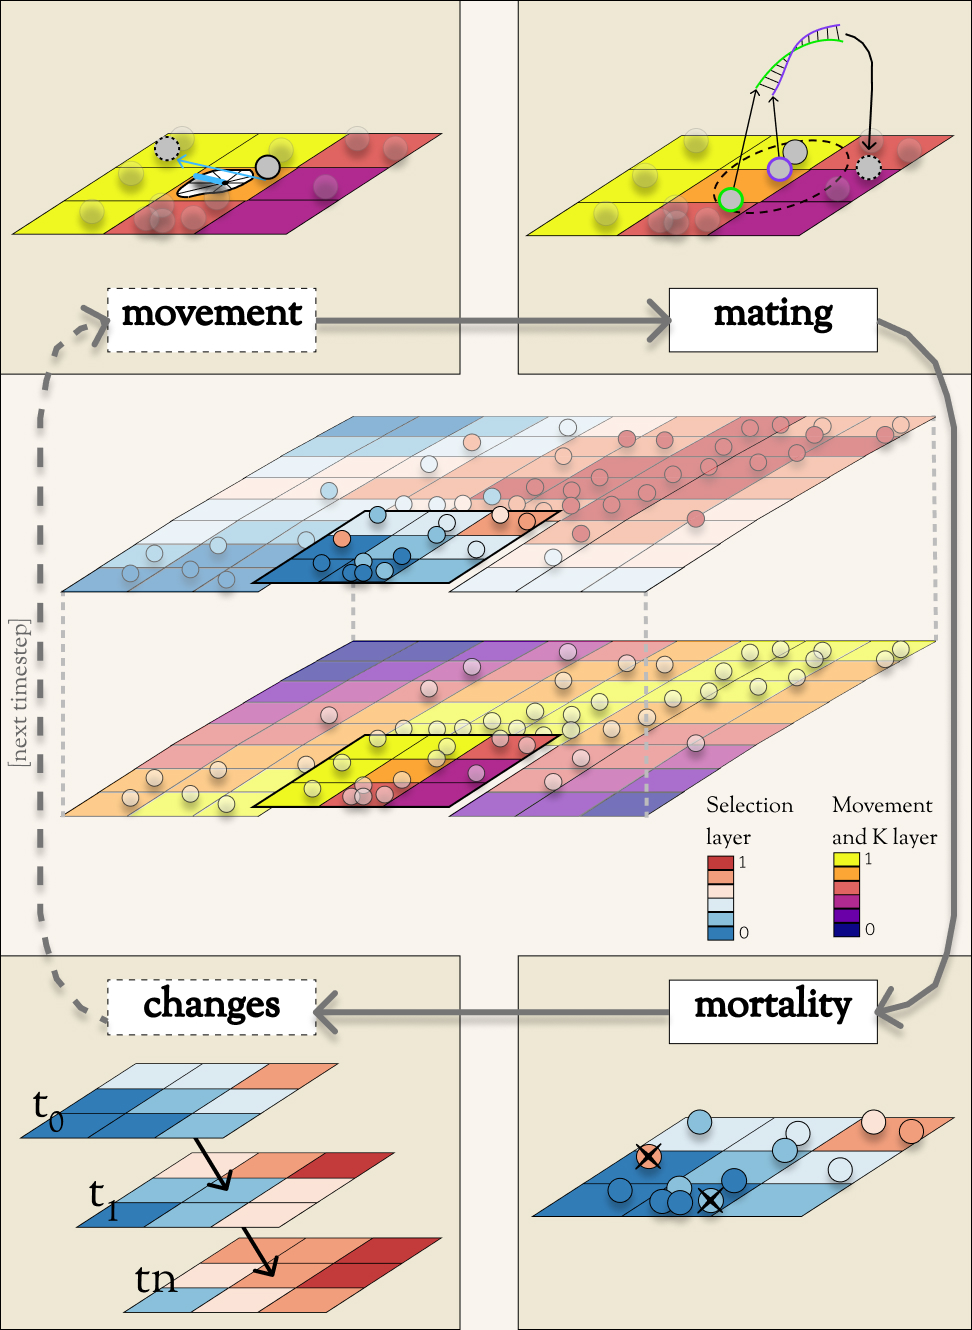
\includegraphics[width=125mm]{./img/final/draft_diagram_CONCEPTUAL.png}
        \centerfloat
        \caption{Geonomics conceptual flow diagram: In the center is a species
                 distributed across a multi-layer landscape---in this case
                 composed of two layers.
                 The upper layer serves as a selection
                 layer for a trait, with both the environmental values and
                 individuals' phenotypic values for the trait indicated by
                 the blue-red colormap.
                 The lower layer serves as both a movement
                 layer and a carrying-capacity (K) layer.
                 Around the landscape is a clockwise representation
                 of the major operations carried out during each timestep,
                 each depicted in its own labeled box. (Dashed-line label boxes
                 indicate optional operations.)
                 \textbf{Movement}: An individual is displaced to a
                 new location along a vector composed of a randomly drawn distance
                 and a randomly drawn direction, with the direction
                 drawn from a circular (Von Mises mixture) distribution determined by
                 the relative permeability of its 8-cell neighborhood.
                 \textbf{Mating}: An individual (outlined in purple) randomly chooses
                 a mate (outlined in green) from among all potential mates located
                 within its mating radius. The mates produce gametes, which become
                 the genome of an offspring individual, which disperses along some
                 randomly drawn vector rooted at its parents' centerpoint.  
                 \textbf{Mortality}: Individuals' probabilities of death are
                 a product of density-dependence (as determined by the comparison
                 between local density and local carrying
                 capacity, according to the logistic growth model) and selection
                 (as determined by the absolute difference between
                 phenotypic values and environmental values on the corresponding
                 selection layers).
                 Death events are Bernoulli draws on these probabilties.
                 \textbf{Changes}: Change events are composed of scheduled,
                 stepwise changes, which occur at the ends of timesteps.
                 These can include both environmental changes (i.e. substitutions
                 of the rasters for certain layers) and demographic changes
                 (not depicted here).}
        \label{fig:flow}
\end{figure}


\begin{figure}[!hp]
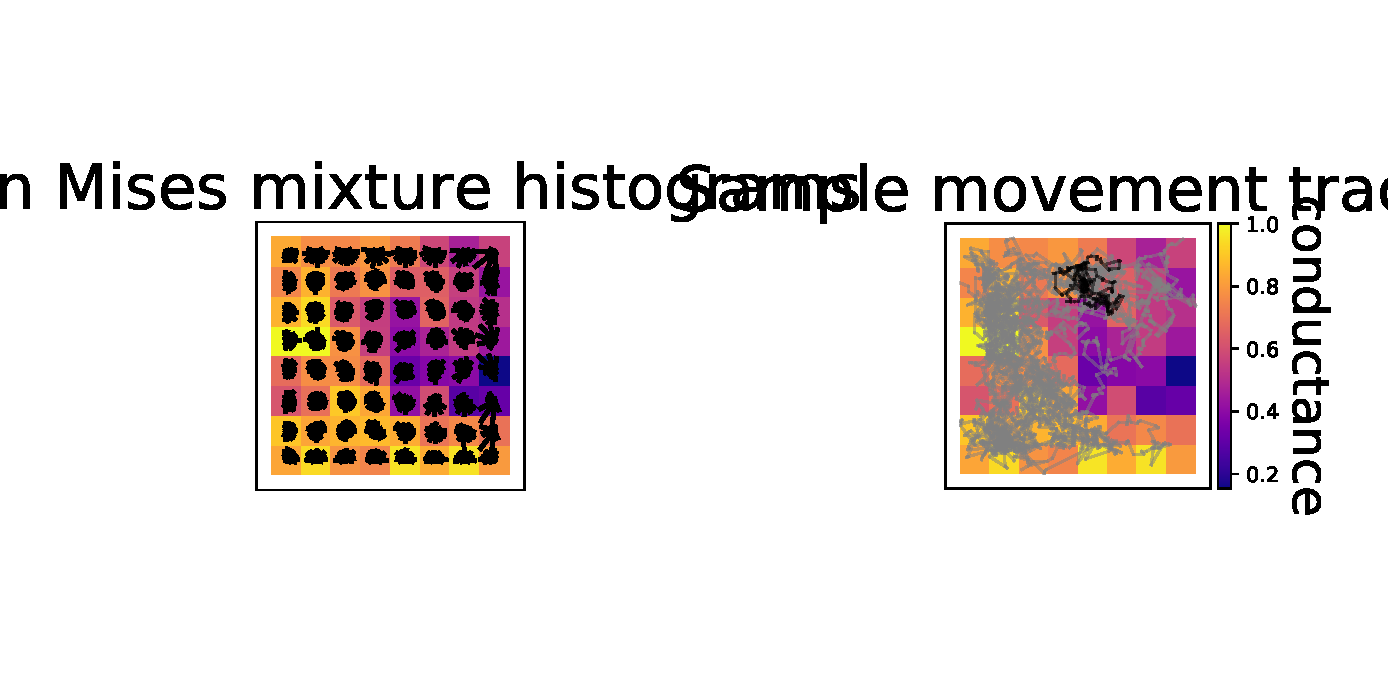
\includegraphics[width=175mm]{./img/final/move_surf.pdf}
        \caption{\textbf{A.} Histograms of the VonMises mixture-distribution approximations
                 underlying a movement surface, plotted over a small landscape
                 layer on which the surface is based.
                 The taller the bar in a histogram, the higher the probability
                 that an individual located on that histogram's cell will move
                 in a direction within the angular neighborhood of that bar.
                 (Plot was produed by the Geonomics method
                 \texttt{model.plot\_movement\_surface}.)
                 \textbf{B.} Examples of movement tracks for 25 individuals
                 randomly selected from a species, moving across
                 the movement surface depicted in A.
                 Each track is 150 steps long, beginning at
                 the individuals' starting locations (white dots),
                 and thickens with each increasing timestep.
                 Individudals' preferential movement toward
                 higher-suitability regions of the landscape
                 (values with environmental values nearer 1) is evident.
                 Occasional migrations between isolated portions of the
                 landscape are also visible.
                 (Plot was produced by the Geonomics function
                 \texttt{gnx.help.param\_help.plot\_movement}.)
                 }
        \label{fig:move_surf}
\end{figure}


\begin{figure}[!hp]
        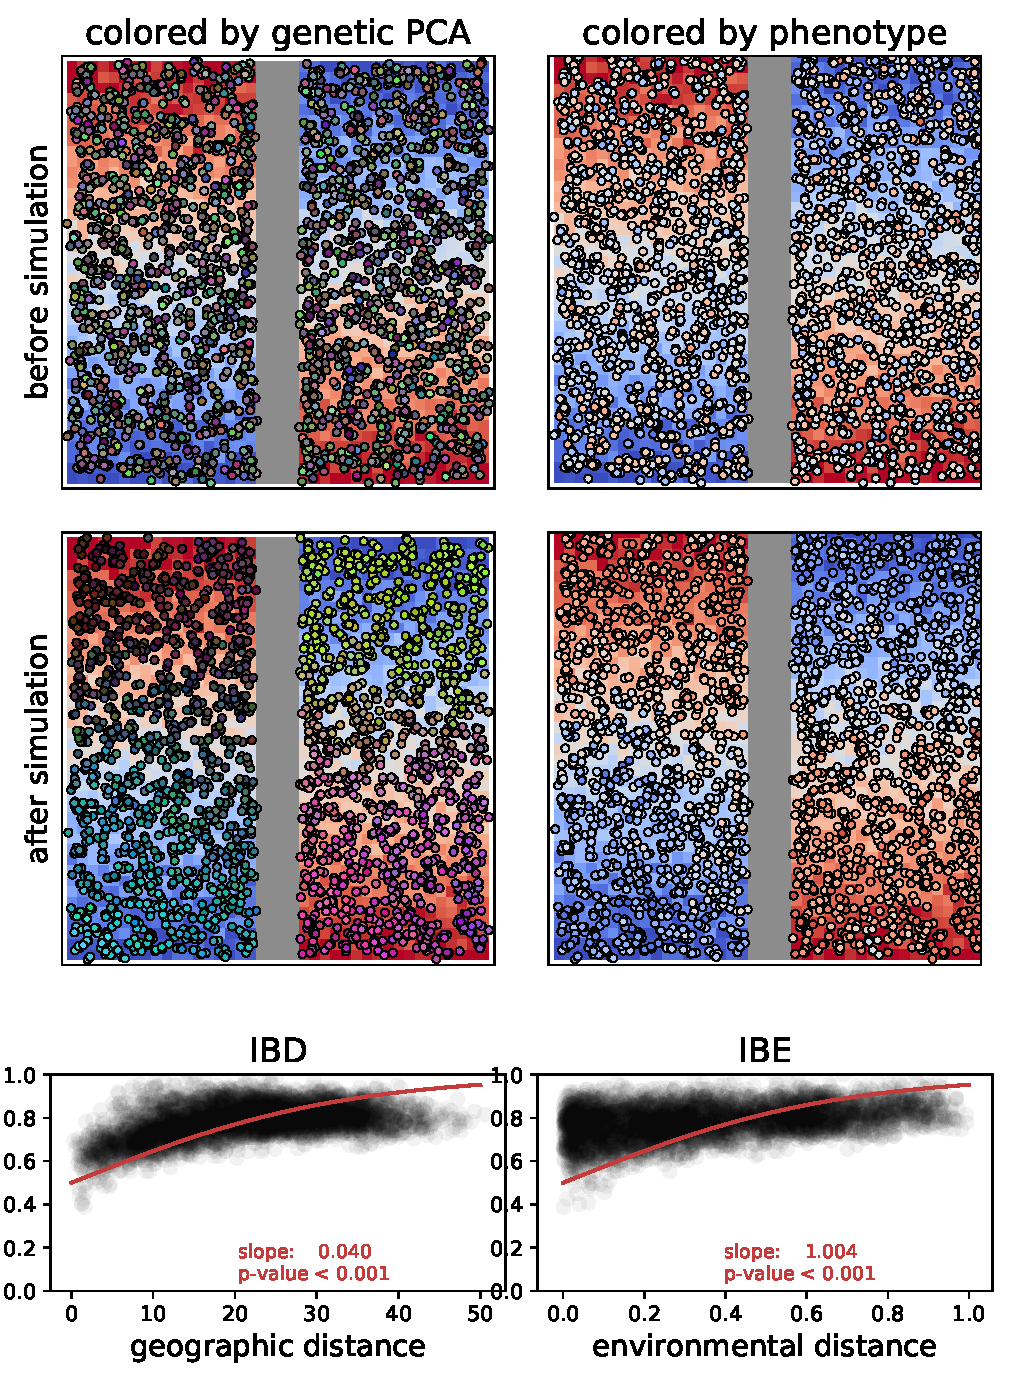
\includegraphics[width=125mm]{./img/final/IBD_IBE.pdf}
        \centerfloat
        \caption{Isolation by geographic and environmental distance. 
                 \textbf{Top two rows}: 
                 Spatial structure in a species evolving on a
                 landscape consisting of 1.) a barrier layer
                 that serves as the species' movement surface
                 (displayed here as the masked band down the landscape center)
                 and 2.) an environmental layer that serves as
                 the selective surface for a 10-locus trait
                 (displayed here as the red and blue regions of the landscape).
                 Species plotted both before (left)
                 and after (right) 1000 timesteps of evolution.
                 Individuals' colors are derived from their scores
                 for the first three PCs of a genetic PCA
                 (with each score scaled to $0\leq value\leq255$,
                 then used to assign RGB values)
                 \textbf{Bottom row:} 
                 Scatter plots of inter-individual pairwise genetic distance
                 (calculated as Euclidean distance in genetic PC space)
                 as a function of Euclidean geographic distance (left)
                 and Euclidean environmental distance (right).}
        \label{fig:IBD_IBE}
\end{figure}



        

\begin{figure}[H]
        \centering
        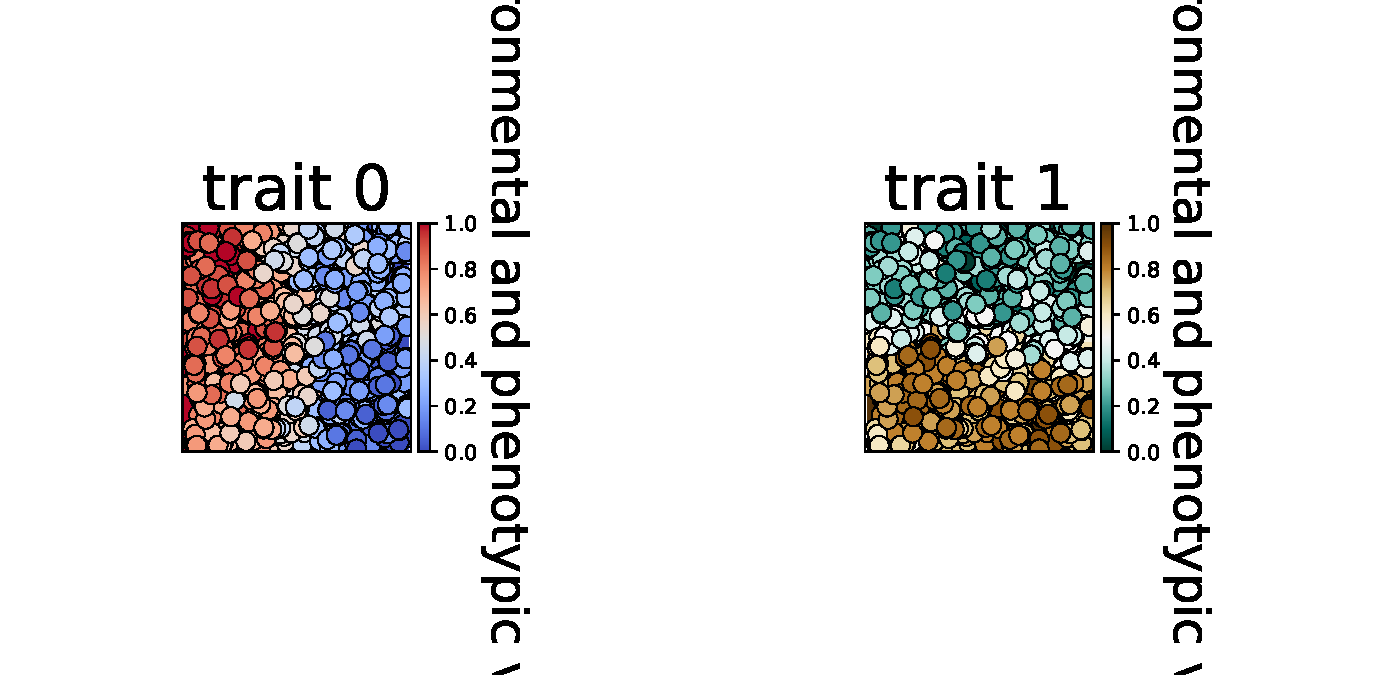
\includegraphics[width=175mm]{./img/final/sim_sel.pdf}
        \caption{Simultaneous-selection test: Results of simulatenous selection
                 on two traits with distinct spatial distributions of selective force.
                 Each trait is controlled by 10 unlinked loci
                 and has a selection coefficient of $\phi = 0.05$.
                 Individuals are colored by phenotype, such that fitter individuals
                 are those whose colors are more similar to their background
                 environmental colors.  (Plots were produced by the
                 Geonomics method \texttt{model.plot\_phenotype}.)}
        \label{fig:sim_sel}
\end{figure}


\begin{figure}[H]
        \includegraphics[width=175mm]{./img/final/YOSEMITE_time_series.pdf}
        \caption{Temperature rasters (top row),
                 habitat rasters (middle row),
                 and rasters of neighborhood-meaned phenotype (bottom row)
                 plotted at timesteps 0 (left column),
                 500 (before beginning of climate change; center column),
                 and 1500 (after climate change; right column)
                 for a species with a 100-gene trait adapted to temperature.
                 (Top- and middle-row plots were produced
                 by the Geonomics method \texttt{model.plot\_phenotype}.)}
        \label{fig:yosemite}
\end{figure}


\begin{figure}[H]
        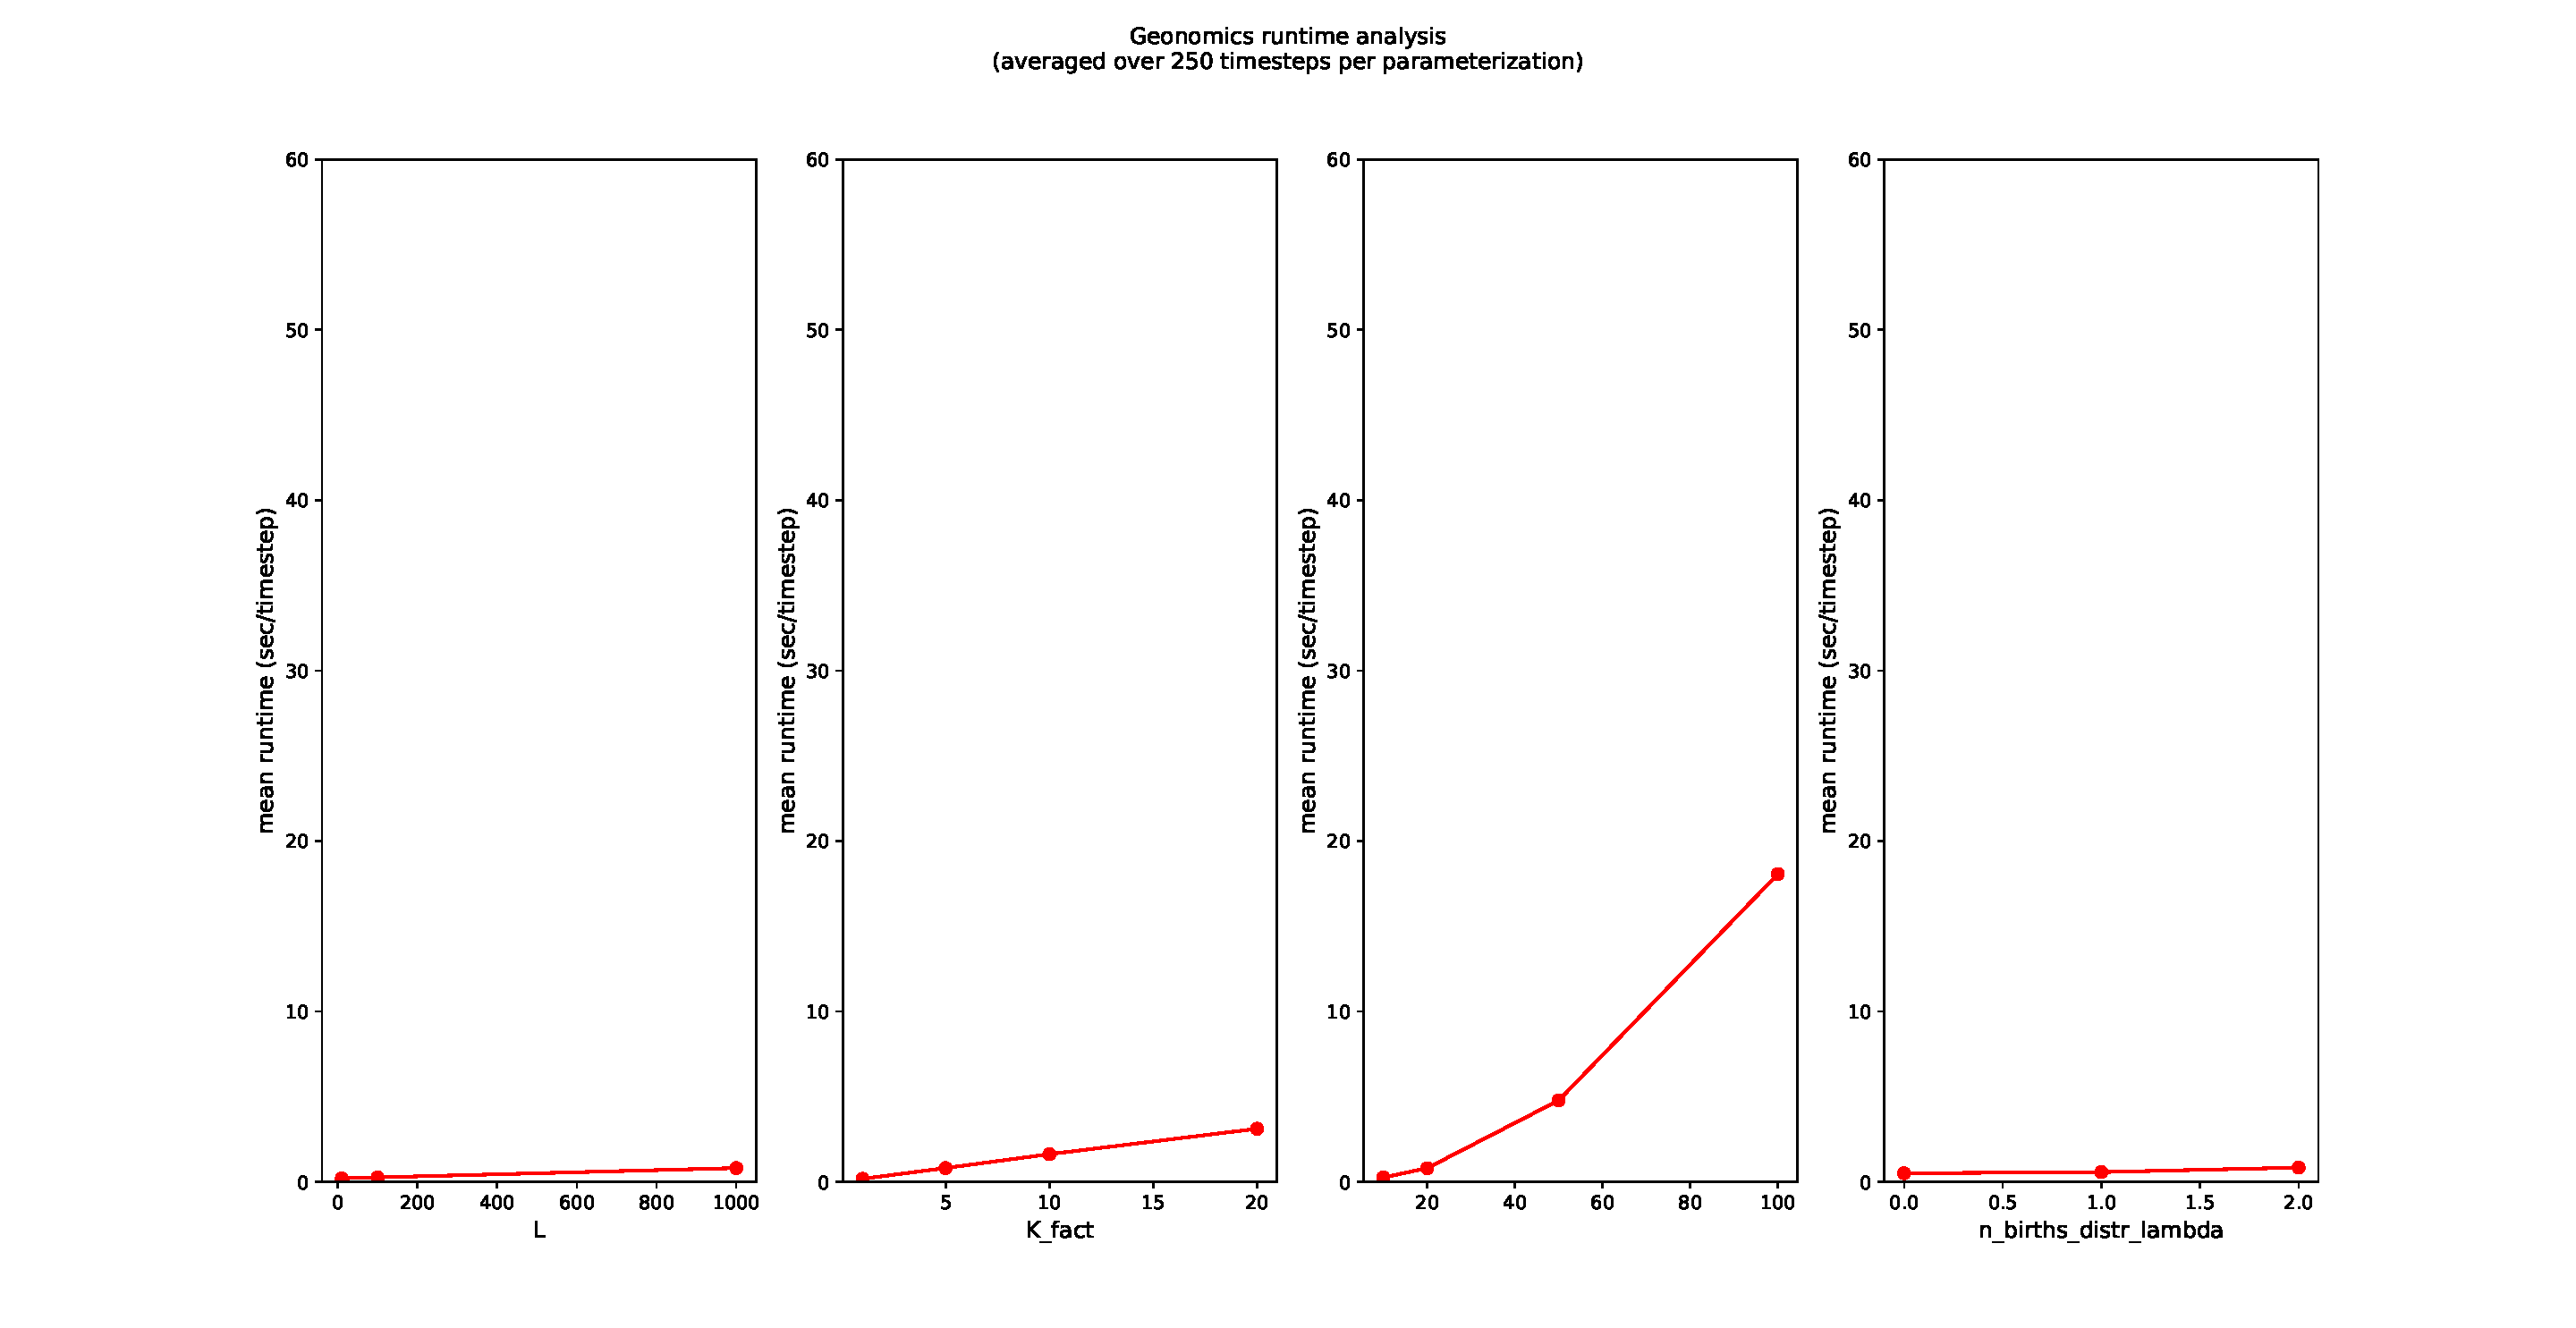
\includegraphics[width=175mm]{./img/final/runtime.pdf}
        \caption{Runtime analysis: average runtime per timestep (in seconds)
                 as a function of various parameters
                 (left to right: \textbf{`K\_factor'}:
                 The factor by which a species' carrying capacity
                 raster is multiplied to determine its local carrying capacities
                 and thus, in sum, its mean total population size;
                 \textbf{`n\_births\_distr\_lambda'}:
                 The $\lambda$ parameter on the Poisson distribution from which
                 the number of offspring per mating event is drawn;
                 \textbf{`dim'}: The dimensions of the simualted landscape;
                 \textbf{`L'}: The length of the simulated genome)}
        \label{fig:runtime}
\end{figure}



\pagebreak
\section{Supplements}

\subsection{Validations tests}
In this section, we briefly review the reasoning and parameterization for each test,
then present the results.
(We discuss only parameters of key importance to each scenario.
Other parameters are set to reasonable values, or left at defaults.
For full details, see the parameters file for a given test.)

All results are as expected, demonstrating a robust ability to reproduce 
population-genetic and population-genomic findings.
Some results show minor deviations from theory.
These artefacts are primarily a resulting of using a simulation framework
designed for complex, spatially explicit models 
to approximate much simpler and, in some cases, aspatial or spatially implicit models.
They artefacts are discussed where applicable.
(The code for all tests is available in the `./tests/validation' directory of the package.)

\subsection{Wright-Fisher test: genetic drift}
The Wright-Fisher model of genetic drift models a fixed-size haploid population that
turns over completely at each timestep (i.e.\ generation).
The population can have any number of independent, biallelic genetic loci.
For each locus, each generation’s allele
frequency is chosen as a binomial random variable, with the number of trials equal to
the population size and the probability of success (i.e.\ of drawing the ‘1’ allele)
equal to the previous generation’s ‘1’-allele frequency.
The mean persistence time for an allele 
(i.e.\ the expected number of generations for which a locus remains segregating) 
is:
\begin{equation}
        \bar{t}(p) = -4N[(1 - p)ln(1 - p) + pln(p)]
\label{eqxn:wf_mean_persist_t}
\end{equation}
where $2N$ is the number of alleles in the population (such that $N$ can
represent the diploid population size) and $p$ is the frequency of either allele
at the locus~\cite{wright,fisher,hartl}.

Clearly, the Wright-Fisher model is much simpler than the sorts of models for which
Geonomics is designed (as are all of the following validations tests)---it is aspatial,
panmictic, features fixed population sizes, models only neutral loci, and so forth. 
Thus, we parameterized Geonomics so as to approximate the model as closely as possible.
To emulate aspatiality and panmixia, we used a population on a homogeneous landscape,
with isotropic movement, and with movement and dispersal distributions
and a mating radius that broadly encompass the diagonal width of the landscape.
To enforce complete generational turnover, we set the
maximum age parameter to 1 timestep. While Geonomics does not maintain constant population
size, we maintained the carrying-capacity raster at a constant, uniform value, thus
maintaining a stationary mean population size. We simulated 100, independent neutral
loci (by setting all interlocus recombination rates to 0.5), with starting '1'-allele
frequencies of 0.5 (although the actual starting frequencies vary slightly around
this value because of sampling error when all individuals' genotypes are drawn binomially).

We ran the Wright-Fisher approximation test for three values of the
carrying-capacity raster (i.e.\ three values of `K\_factor'), hence for three mean
population sizes. For each mean population size (calculated as the harmonic mean,
to account for stochastic fluctations around the carrying capacity), we compared
mean persistence time to that
expected by theory, according to equation~\ref{eqxn:wf_mean_persist_t} in the previous paragraph. As can be
seen in Figures~\ref{fig:wf_trajs} and~\ref{fig:wf_persist_vs_popsize}, the results are a close match to theory.


\subsection{Bottleneck test: population dynamics}
Because drift is a stronger evolutionary force in smaller populations,
drift accelerates in shrinking populations. 
If a population undergoes a bottleneck event, the overall effect of drift on the population
during that time is expected to be larger than a constant-size population of equivalent
starting size would experience during that time. 
Thus, mean fixation time should decrease in a bottlenecked population
relative to a constant-size comparison population.

As with the Wright-Fisher model, we used a homogeneous landscape with broad distributions
for movement and dispersal and with a mating radius that encompasses the full landscape
to emulate aspatiality and panmixia. To simulate a bottleneck event,
we created a custom change event in which the population's carrying-capacity raster
is reduced to 30\% of its initial value for 50 timesteps (from the 200th to 250th),
then returned to its initial value for the remainder of the simulation
(through the 2500th timestep).

Figure~\ref{fig:bottleneck} shows a clear signal of drift acceleration during the bottleneck event.


\subsection{Stepping-stone test: population subdivision and genetic differentiation}
The stepping-stone model, or one-dimensional island model, is a spatially implicit model.
It models a series of subpopulations, arranged along a straight line,
with migration between all neighboring pairs.
As a combined result of divergence by drift and homogenization
by effective migration, subpopulations are expected to reach
a stationary level of genetic differentiation---migration-drift equilibrium. 
Theory provides the expected pairwise genetic differentiation
between a pair of subpopulations at equilibrium as:
\begin{equation}
        F_{ST} = \frac{1}{1 + 4Nm}
\label{eqxn:F_ST_as_fn_of_mig}
\end{equation}
where $N$ is the population size and $m$ is the per-generation migration rate,
such that $Nm$ can be interpreted as the per-generation number of migrant
individuals~\cite{hartl}.

To approximate the stepping-stone model, we created a Landscape Layer with a diagonal
of six equally spaced islands (1.0-valued cells) embedded in a `sea' of 0.0-valued cells.
We used this layer as the carrying-capacity raster (Figure~\ref{fig:stepstone_pop_and_Fst_mig_expecs}, left).
We set the mating radius to encompass an individual's current island, but no neighboring islands.
We parameterized dispersal to be very local to parents' midpoints, and
parameterized movement distance to be strongly right-skewed, such that
the long-distance movement events leading to migration are uncommon.
We ran the simulation for 5000 timesteps.

Because Geonomics does not model discrete populations, it does not stipulate
migration rates between discrete locations on the Landscape.
Thus we manually tracked the number of migration events during each timestep,
for all possible directional migration events (i.e.\ for all permutations of island pairs),
then used that data to calculate all mean migration rates.
With those values, we solved equation~\ref{eqxn:F_ST_as_fn_of_mig},
then compared the resulting $F_{ST}$ expectations to the observed values
(calculated from the simulated data using two common methods;
see Figure~\ref{fig:stepstone_pop_and_Fst_mig_expecs} for details).

All island populations were at dynamic equilibria around the same mean size,
and results demonstrate that the model approached migration-drift equilibrium,
as expected by theory (Figure~\ref{fig:stepstone_Fst_by_dist}).
Estimated migration rates and $F_{ST}$ values qualitatively match theoretical expectations:
mean migration rate drops off precipitously at greater than one island's distance apart, 
and genetic differentiation increases to approximate saturation.
Values of $F_{ST}$ consistently undershoot the values expected based on estimated
migration rates, however, because subpopulations have yet to approach fixation
at most loci (which is the expectation implied by expected $F_{ST}$ values
close to 1).


\subsection{Contrasting-habitat test: adaptive divergence}
In a population divided between two opposite selective environments, if there is
standing genetic variation for a biallelic locus controlling the trait responding
to those environments, then theory predicts that the two subpopulations will diverge at
that locus as each moves toward its respective adaptive peak.
The rate at which divergence should occur depends on the relative strengths
of two opposing evolutionary forces: natural selection, which causes divergence,
and gene flow from migration, which causes homogenization. 
The rate of allele frequency change
in either subpopulation at timestep t is expressed as:
\begin{equation}
        \delta{q} = \frac{-spq[q + h(p - q)]}{1 - sq(2hp + q)} + m_{i}q^{*} - m_{o}q
\label{eqxn:rate_allele_freq_change}
\end{equation}
where $q$ and $p$ are the frequencies of the deleterious and beneficial alleles
in the subpopulation, $s$ is the selection
coefficient against the homozygous recessive phenotype, $h$ is the degree of dominance
of the recessive allele, $m_{i}$ and $m^{o}$ are the migration rates into and out of
the subpopulation being analyzed, and $q^{*}$ is the frequency of the recessive allele
in the alternative subpopulation~\cite{hartl}.

This model, much like the stepping-stone model, is spatially implicit.
To approximate this, we created a landscape with two layers.
The first was divided into two equal-sized halves, one valued at 0.0, the other at 1.0;
this layer was used as the layer driving natural selection.
The second was valued uniformly at 1.0; this was used as the carrying-capacity raster
(thus setting uniform population density across the Landscape and determining,
in sum, the overall carrying capacity of the landscape).
We created one monogenic trait whose position was randomly chosen within a 
genomic architecture of 100 independent (i.e.\ unlinked) loci.
We ran the model for 1000 timesteps for each of three values of the parameter phi
(identical to \emph{s} in equation~\ref{eqxn:rate_allele_freq_change}): 0.1, 0.05, and 0.01.
Given that Geonomics does not employ express migration rates,
we tracked the number of migration events (betwen the two contrasting halves of the first layer)
during each timestep, then used that data to solve equation~\ref{eqxn:rate_allele_freq_change}.

Results depict clear local adaptation to each of the two halves of the landscape,
with opposite-phenotype bleedover and heterozygote births occuring along
the border between the two habitats (Figure~\ref{fig:div_pop} right).
Allele trajectories in each half of the environment follow qualitatively 
the increasing and saturating trajectories expected by theory,
but reach consistently more extreme allele frequencies than expected (Figure~\ref{fig:div_freqs}, left).


\subsection{Cline test: local adaptation}
In a clinal model, a population adapts locally across an environmental gradient,
which is characterized by the extremes of its environmental values and its steepness
(i.e.\ the instantaneous rate of environmental change along it).
Local adaptation across this gradient will generate a cline,
i.e.\ a geographic gradient in allele frequency
(though natural selection is not the only way a cline could be produced).
The clinal pattern is only expected for loci that underlie the trait underoing
selection along the cline (and loci in linkage).
Unlinked loci have no long-term clinal expectation
(though they could initially be swept along with the selective locus adaptation,
and any number could continue to show spurious concordant clinal variation).
To detect clinally adapted loci, we can fit cline curves to the allele-frequency
variation across the environmental gradient for all loci,
with the expectation that the clines fit to adaptive loci will mirror the gradient.
Numerous equations have been used to fit clines, but one of the most common
is the sigmoidal \emph{tanh} function:
\begin{equation}
        p_{x} = \frac{1}{2}(1 + \tanh[\frac{2(x - c)}{w}])
\label{eqxn:cline}
\end{equation}
where $p$ is the frequency of the reference allele at position $x$ along the cline,
$c$ is the centerpoint of the cline (such that $p_{x=c} = 0.5$), and $w$ is the 
`width', which is defined as $w = \frac{1}{slope}$ at centerpoint $c$~\cite{porter}. 

To implement the cline model in Geonomics, we created a landscape with two layers.
The first layer was an environmental layer---a symmetrical, non-linear gradient
between 0-valued and 1-valued halves (see raster in both halves of Figure~\ref{fig:cline}).
The second was a uniformly valued habitat-quality layer, used to set a uniform
population density and thus determine the global carrying capacity.
We created a monogenic trait whose locus was randomly placed within a
genomic architecture of 100 independent loci.
The trait had a \emph{phi} (i.e.\ \emph{s}) of 0.01,
with the gradient layer serving as its selective force.

We ran the cline model for 2500 timesteps, then used a numerical optimization function
(in Python's \texttt{scipy} package~\cite{scipy}) to fit equation~\ref{eqxn:cline} for all loci.
We plotted all fitted clines on top of the first landscape layer,
with the cline for the one selective locus highlighted.
The selective locus consistently and clearly stands out as the only locus with a cline
matching the expectation (i.e.\ mirroring the environmental gradient; Figure~\ref{fig:cline_fits}),
and results show an obviously locally adapted population, with a zone of hybridization
and phenotypic spillover surrounding the cline's center (Figure~\ref{fig:cline_pop}).
Furthermore, for a family of regression models of environmental value
on genotype for all loci, after Bonferroni correction for multiple testing,
the selective locus is consistently significant and the most significant 
(though other loci produce false-positive results, albeit with considerably larger p-values).
INCLUDE AND SHOW THESE REGRESSION RESULTS?


\subsection{Selective sweep test: genetic hitchhiking}
Genomic context and linkage add important complication to models of molecular evolution.
The most basic model of selection with linkage is that of the selective sweep:
a beneficial mutation occurs in a population, falling on a random genomic background,
then rises in frequency because of its selective advantage until it becomes fixed,
pulling up the frequency of the surrounding haplotype block in the process.
But as the haplotype block increases in frequency it is nevertheless subject to recombination,
which gradually erodes it symmetrically around the beneficial mutaiton.
Thus the selective-sweep model predicts that once a beneficial mutation occurs
---as long as it is not lost early on by chance---
it and the haplotype block around it will rise in frequency,
the mutation will eventually fix, potentially with some core block around it,
but the rest of the block will erode fade over time.
The haplotype block should be clearly visible in genomic data,
where it will manifest as a genomic region of reduced diversity and heterozygosity,
centered on the mutation.

To implement the selective sweep model in Geonomics, we again created a model
approximating an aspatial, panmicitic population (see Wright-Fisher test for details).
We created a single, monogenic trait with a \emph{phi} (i.e.\ \emph{s}) of 0.15.
The trait's locus was manually set to position 50,
such that it was at the center of the the 101-locus genomic architecture.
We manually set the starting '1'-allele frequency at this locus to 0.0,
but set the trait to selected upon by the landscape's first and only layer
(a uniformly 1-valued raster), such that all individuals began the model
equally ill-fit (i.e.\ with a fitness value of $1 - \phi = 0.85$).
After burning the model in, we iteratively chose a random individual,
introduced a '1'-mutation in their genome at locus 50, ran the model for 50 timesteps,
and checked whether the '1' allele had reached a frequency greater than 0.05 by that time.
We iterated until that check was passed, at which point we declared the mutant allele
`established' and continued to run the model until 2500 timesteps
after the mutant reached fixation.
At three timepoints during that model we calculated and recorded
genome-wide nucleotide diversity using a sliding-window approach.

Geonomics realistically emulated the behavior of a selective sweep.
The adaptive phenotype (the '1'|'1' genotype, plotted as white
on a white environmental background; in Figure~\ref{fig:sweep_pop_and_nuc_div}, top row)
clearly emerged in a region surrounding the mutation's origin,
then spread rapidly throughout the population.
The population's mean fitness increased quickly from 0.85
(the universal fitness value before the mutation was introduced) to 1.00
(the universal fitness value after the sweep was complete;
Figure~\ref{fig:sweep_mean_fit}).
The linkage block around the sweeping locus was clearly visible
as a region of depressed nucleotide diversity, which became more pronounced
as the sweep went to completion, then slowly eroded as a result of recombination
of the mutant haplotype's alleles onto non-mutant backgrounds
(Figure~\ref{fig:sweep_pop_and_nuc_div}, bottom row).




\bibliographystyle{plain}
\bibliography{articles_etc,pkgs}



\pagebreak
\section{Figures and Captions}


\begin{figure}[ht]
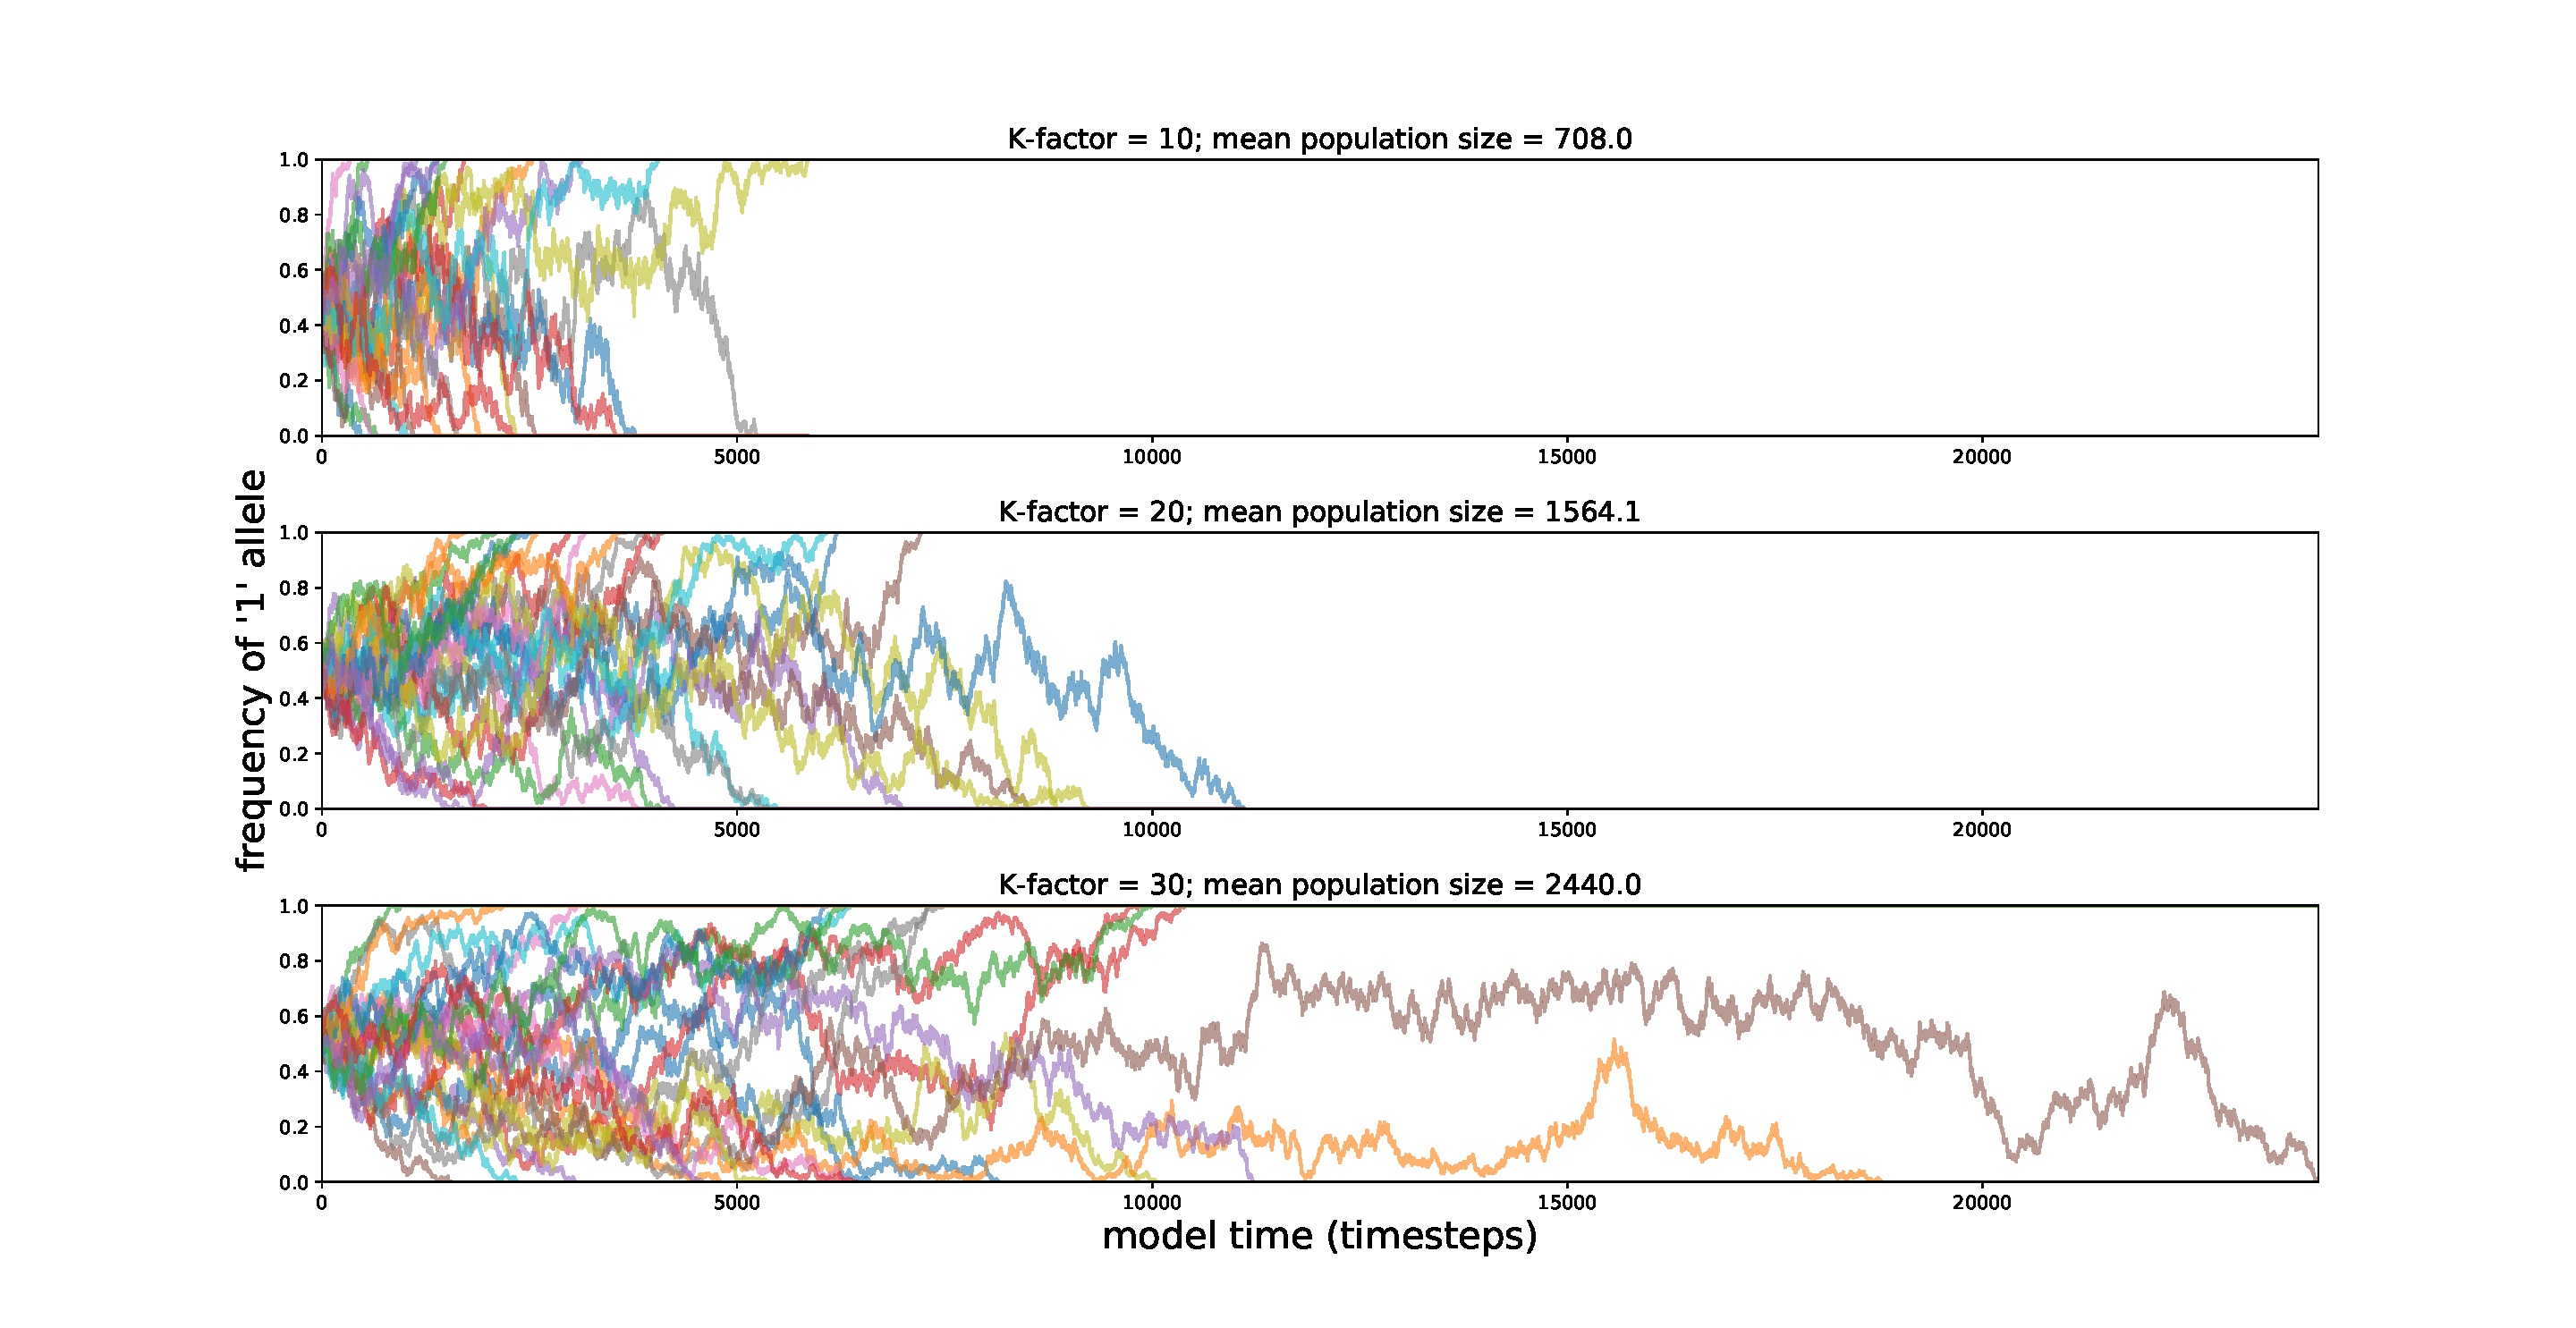
\includegraphics[width=175mm]{./img/final/WF_allele_trajectories.pdf}
        \caption{Wright-Fisher test: Trajectories for the frequencies of
                 the `1'-alleles at each of 25 loci (one line per locus)
                 in a Wright-Fisher model without mutation.
                 Models were run for each of three mean population sizes
                 (as determined by each of three fixed values for the
                 `K\_factor' parameter, the factor by which the 0-1
                 carrying-capacity raster is multiplied in order to
                 define local carrying capacities and thus total population
                 size).
                 Models were run until all loci fixed.}
        \label{fig:wf_trajs}
\end{figure}


\begin{figure}[!p]
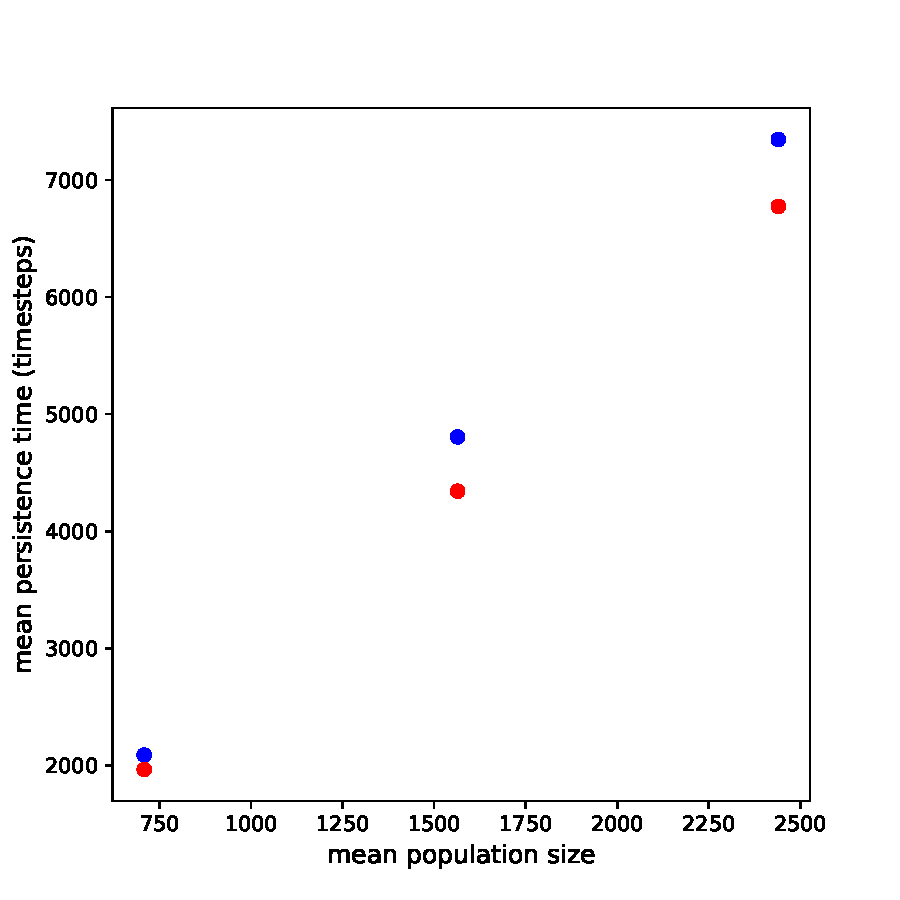
\includegraphics[width=150mm]{./img/final/WF_mean_persist_vs_pop_size.pdf}
        \caption{Wright-Fisher test: Mean persistence time across all loci
                 as a function of harmonic mean population size,
                 compared between predictions based on
                 Equation~\ref{eqxn:wf_mean_persist_t} (red dots)
                 and observed values (blue).}
        \label{fig:wf_persist_vs_popsize}
\end{figure}


\begin{figure}[!p]
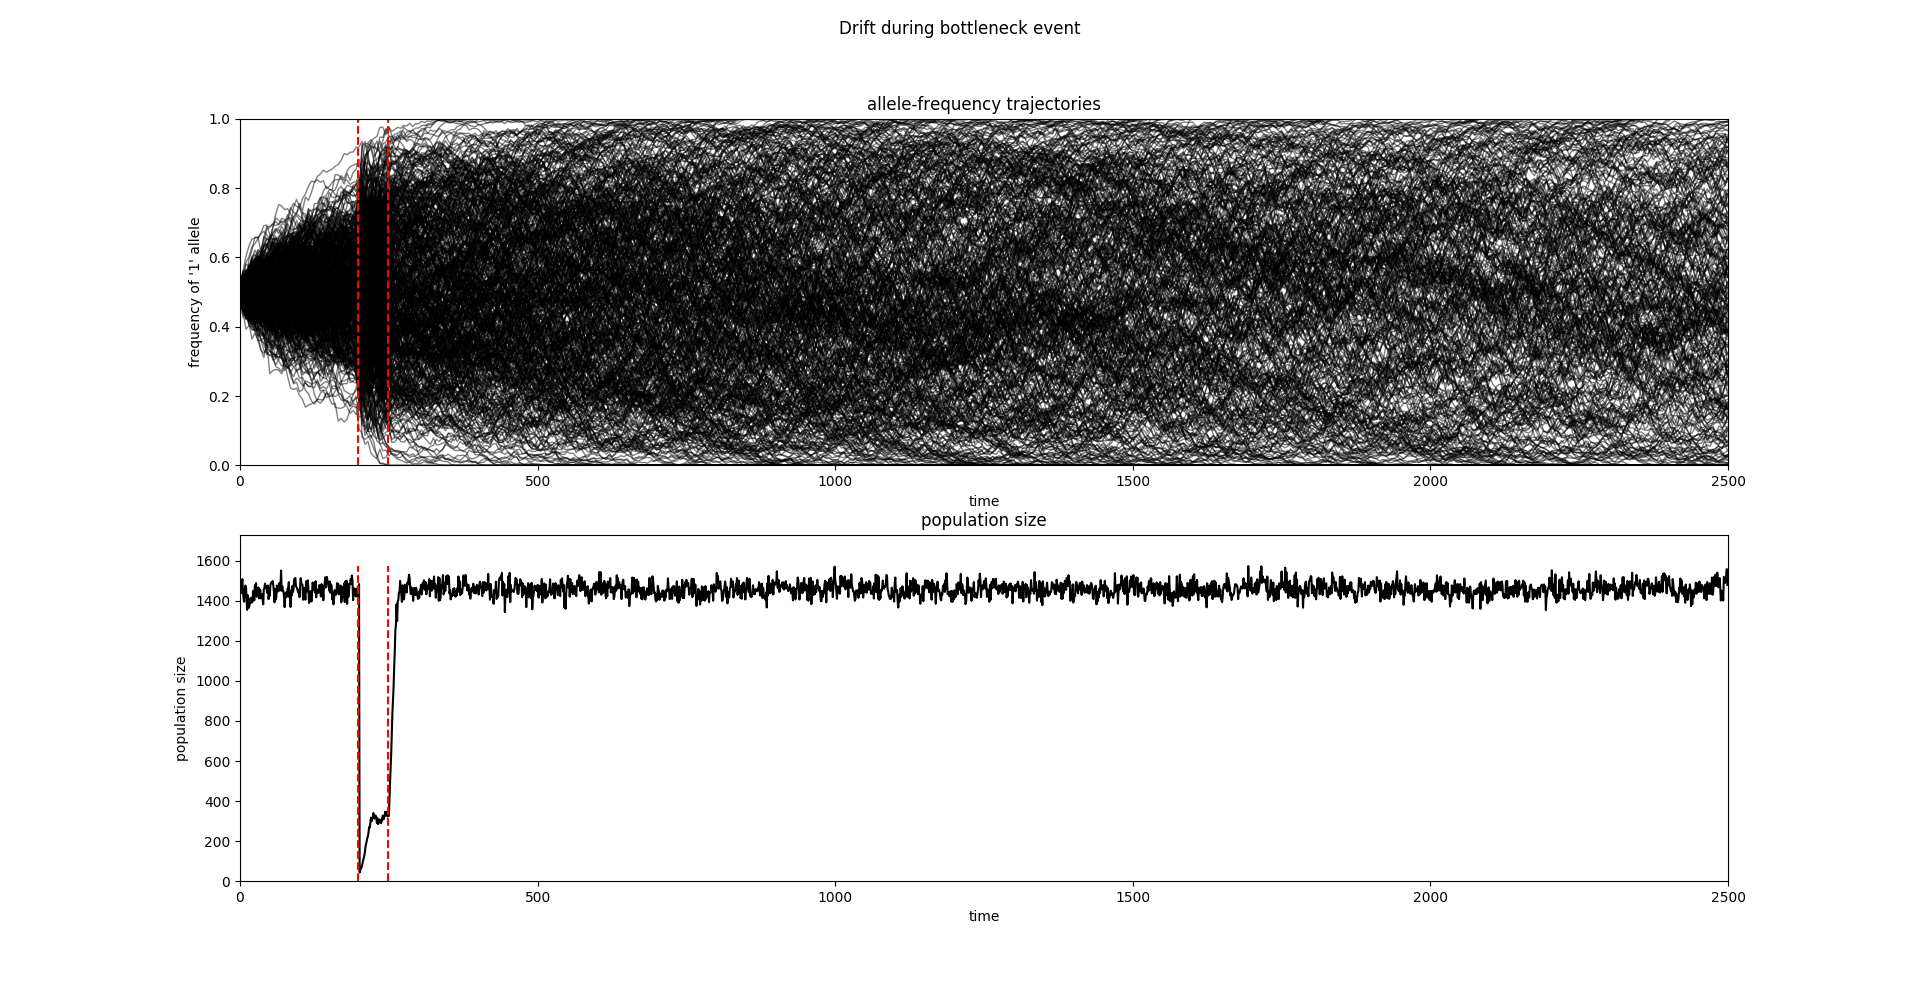
\includegraphics[width=175mm]{./img/validation/bottleneck/alleles_seem_to_take_too_long_to_fix.png}
        \caption{Bottleneck test: 1-allele frequencies (top)
                 and population size (bottom) as a function of time,
                 for a model 2500 timesteps long with a 50-timestep bottleneck}
        \label{fig:bottleneck}
\end{figure}


\begin{figure}[!p]
        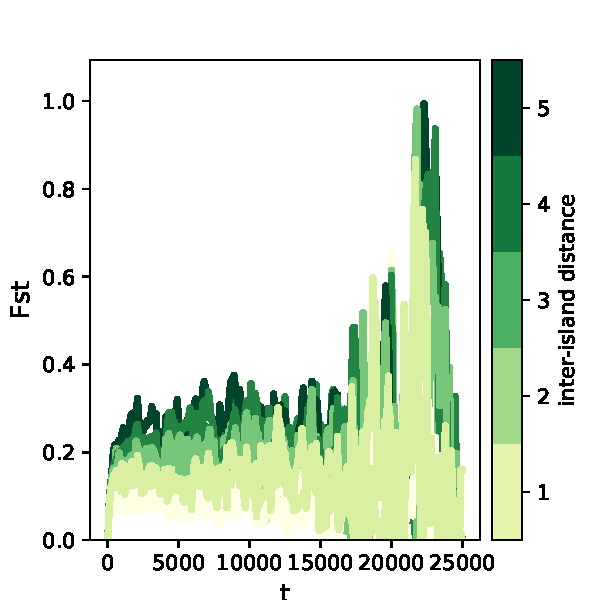
\includegraphics[width=175mm]{./img/final/STEPPING_STONE_Fst_over_time}
        \caption{Stepping-stone test: $F_{ST}$ over model time,
                 plotted across increasing inter-island distances
                 (from yellow to green)}
        \label{fig:stepstone_Fst_by_dist}
\end{figure}


\begin{figure}[!p]
        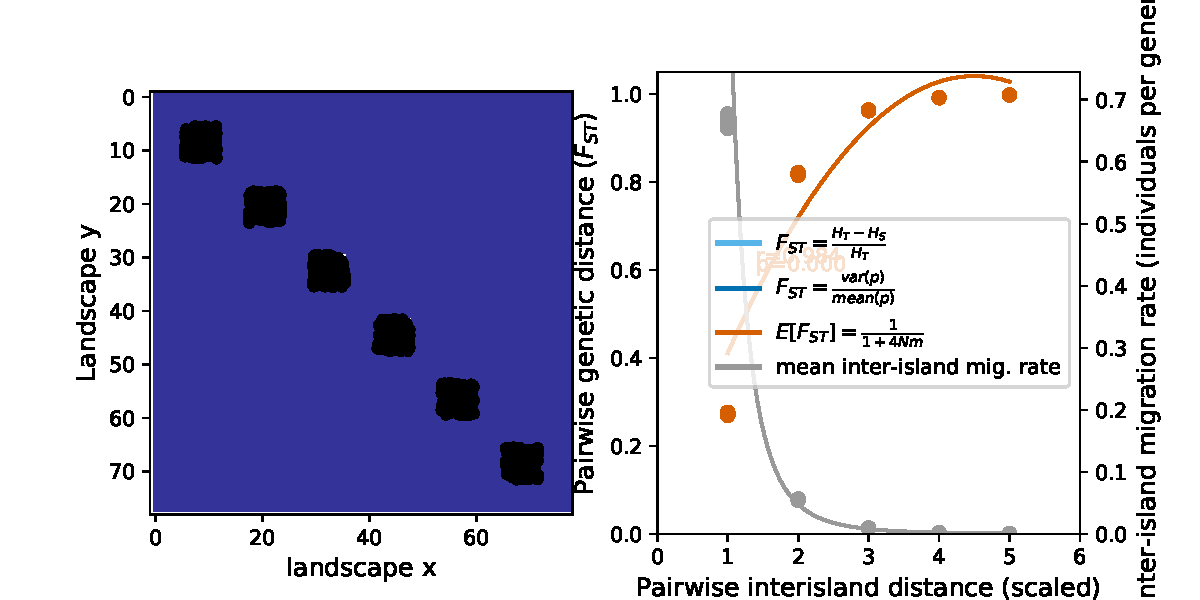
\includegraphics[width=190mm]{./img/final/STEPPING_STONE_pop_plot_and_Fst_vs_mig_rate.pdf}
        \caption{Stepping-stone test: Left: Map of all 6 islands' populations
                 at the end of the simulation;
                 Right: Pairwise $F_{ST}$
                 (left y-axis; calculated by 3 different formulae, indicated in legend)
                 and inter-island migration rate (right y-axis)
                 as a function of inter-island distance;
                 $R^{2}$ values and p-values result from quadratic regressions
                 of $F_{ST}$ values on inter-island distance and
                 log-log regression of mean migration rate on inter-island distance.
                 (Left plot was produced by the Geonomics method
                 \texttt{model.plot}.)}
        \label{fig:stepstone_pop_and_Fst_mig_expecs}
\end{figure}


\begin{figure}[!p]
        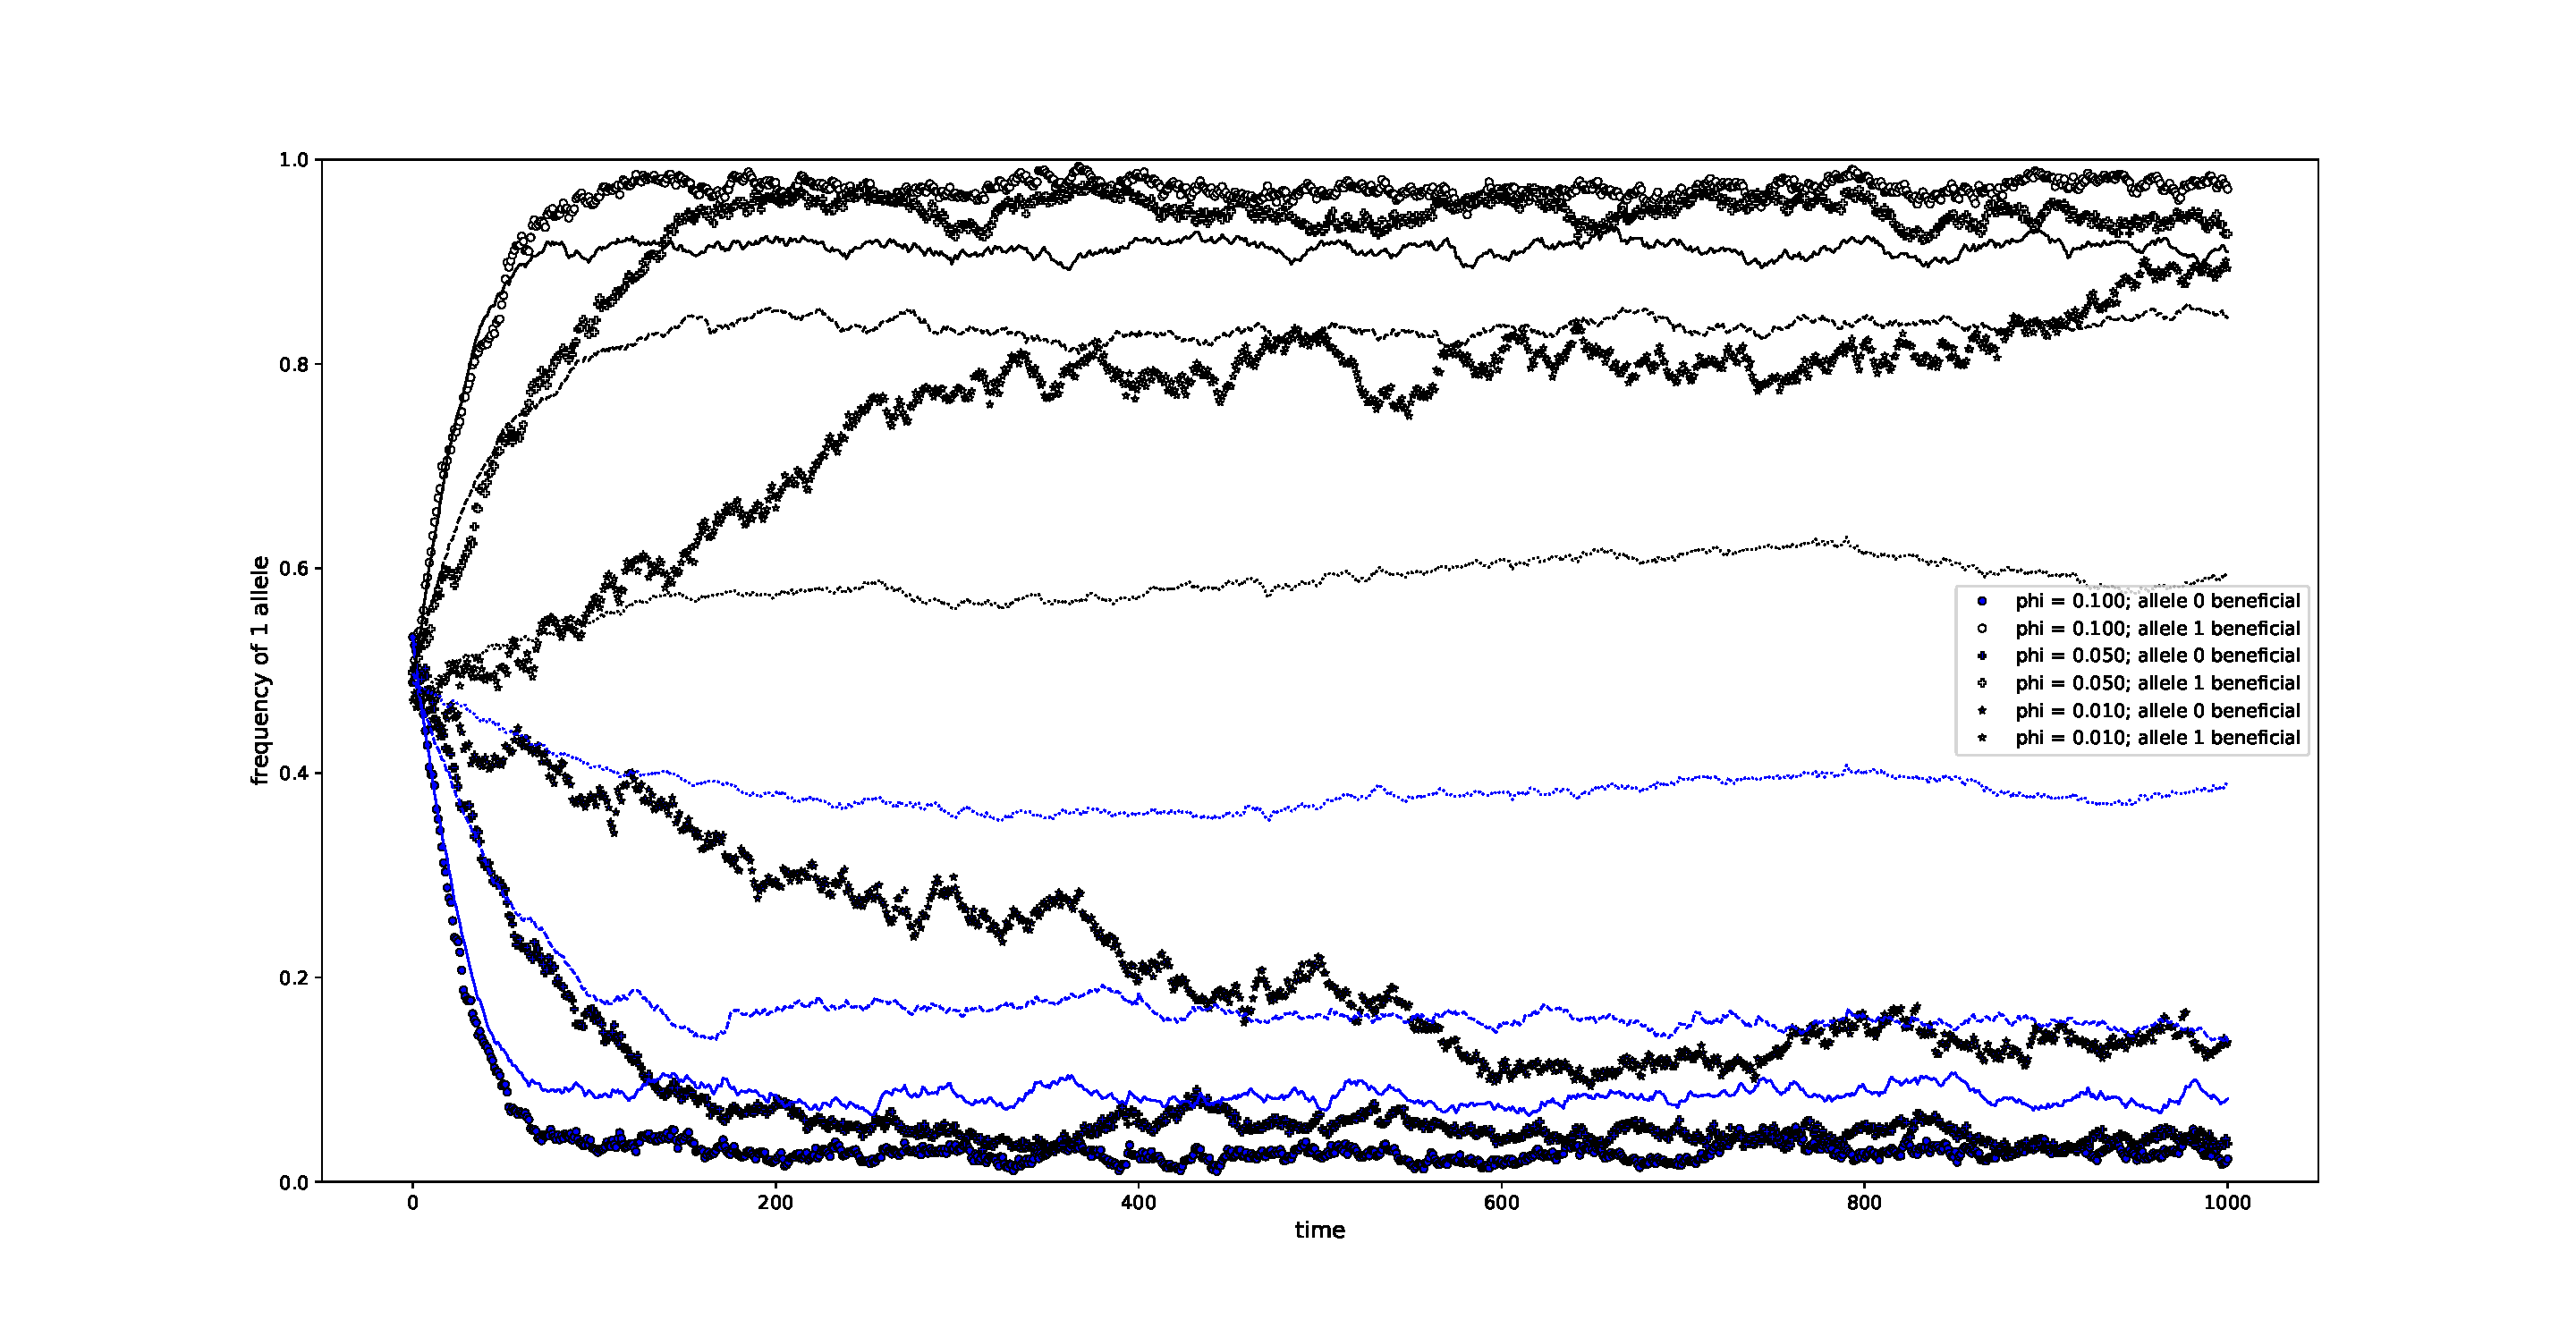
\includegraphics[width=175mm]{./img/final/DIVERGENCE_allele_freqs.pdf}
        \caption{Divergence test: Observed (markers) versus predicted (lines)
                 allele-frequency trajectories for two contrasting habitats
                 (blue = 0.0-valued; white = 1.0-valued),
                 across models with three selection coefficients
                 ($\phi$ = 0.01: stars; 0.05: crosses; 0.10: circles)}
        \label{fig:div_freqs}
\end{figure}


\begin{figure}[!p]
        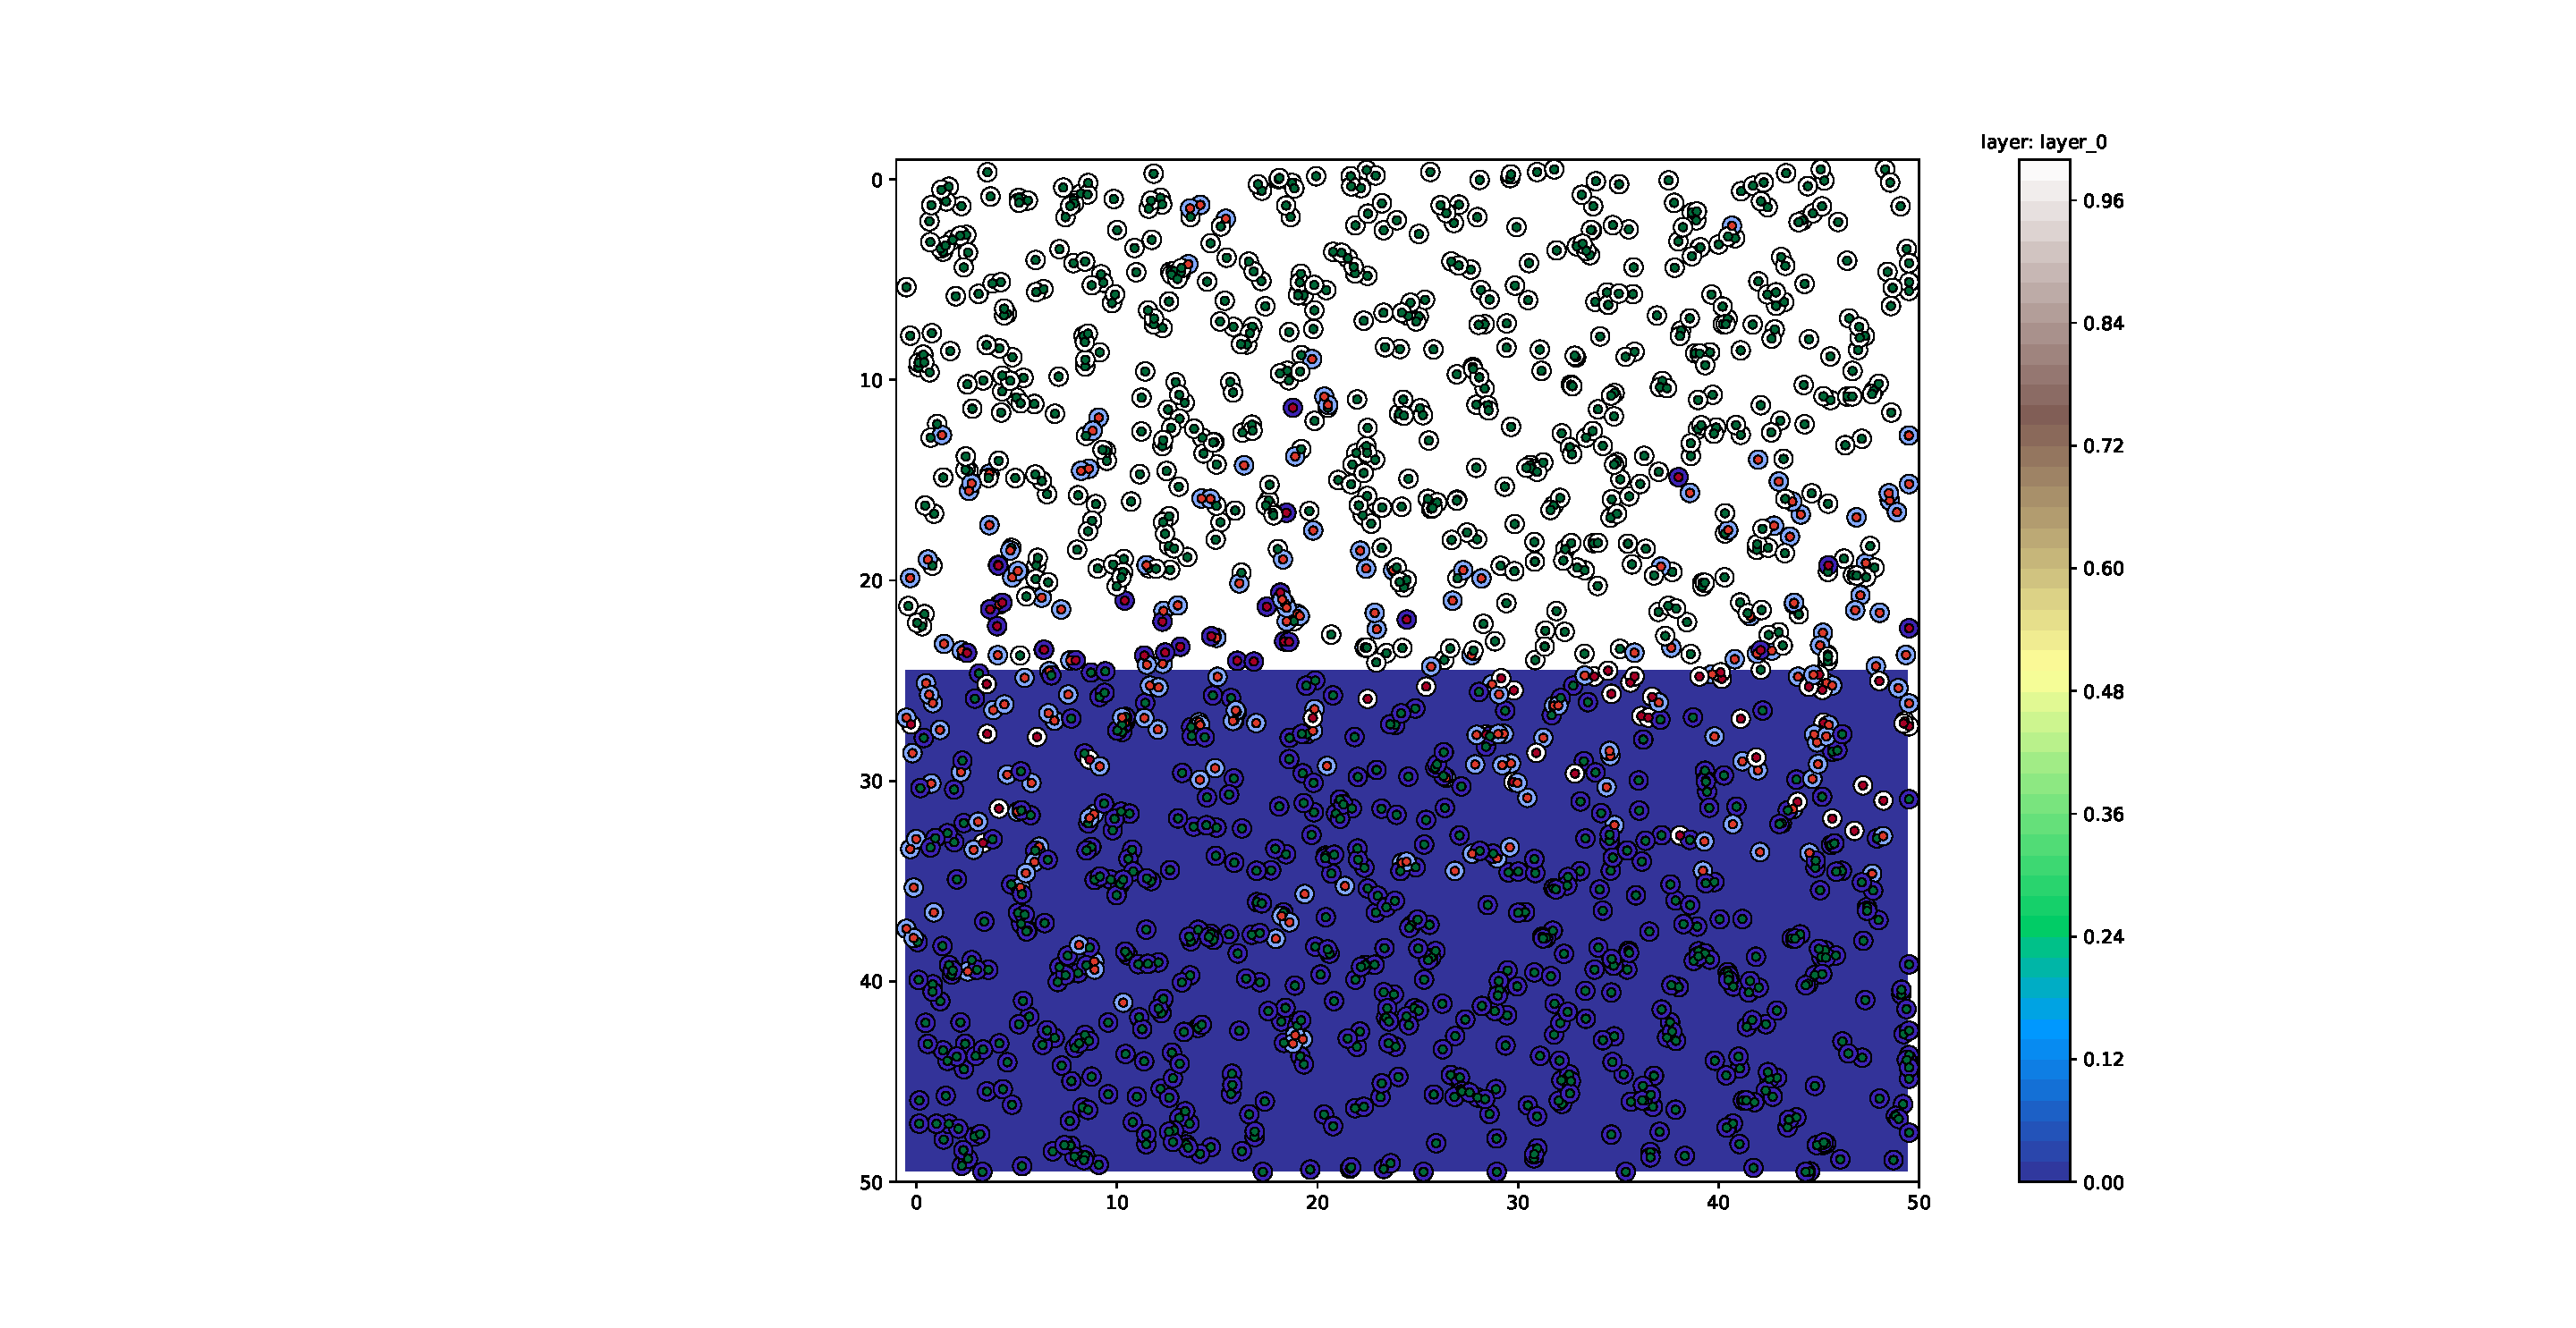
\includegraphics[width=175mm]{./img/final/DIVERGENCE_pop_plot.pdf}
        \caption{Divergence test: Map of the population after
                 spatially divergent selection at $\phi$ = 0.10.
                 Individuals are plotted on top of the selective landscape layer
                 (vertically divided into white and blue halves).
                 They are colored by phenotype (outer circles;
                 color ranges between white and dark blue,
                 representing the optimal phenotypes on
                 their color-matched environmental backgrounds)
                 and by fitness (inner circles; increasing from red to green).
                 (Plot was produced by the Geonomics method
                 \texttt{model.plot\_fitness}.)}
       \label{fig:div_pop}
\end{figure}



\begin{figure}[!p]
        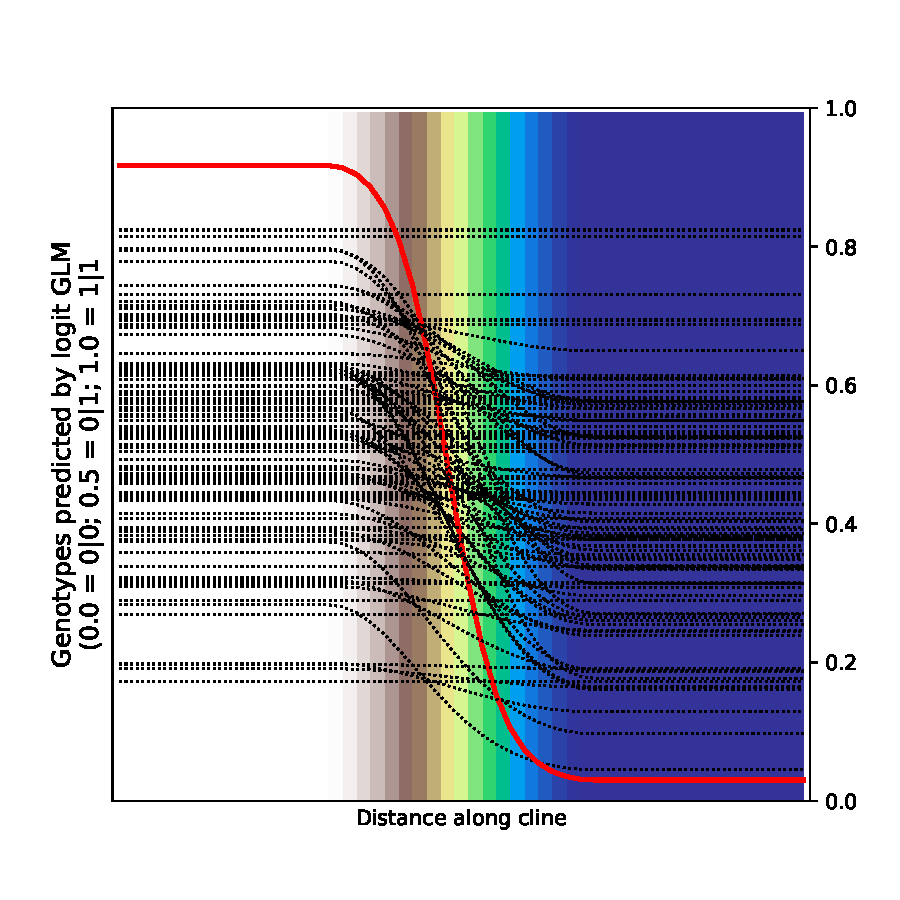
\includegraphics[width=175mm]{./img/final/CLINE_fitted_clines.pdf}
        \caption{Cline test: Plot of allele-frequency clines
                 (neutral loci in black, selective locus in bold red)
                 against the selective landscape layer
                 (horizontal gradient from blue to white)}
        \label{fig:cline_fits}
\end{figure}



\begin{figure}[!p]
        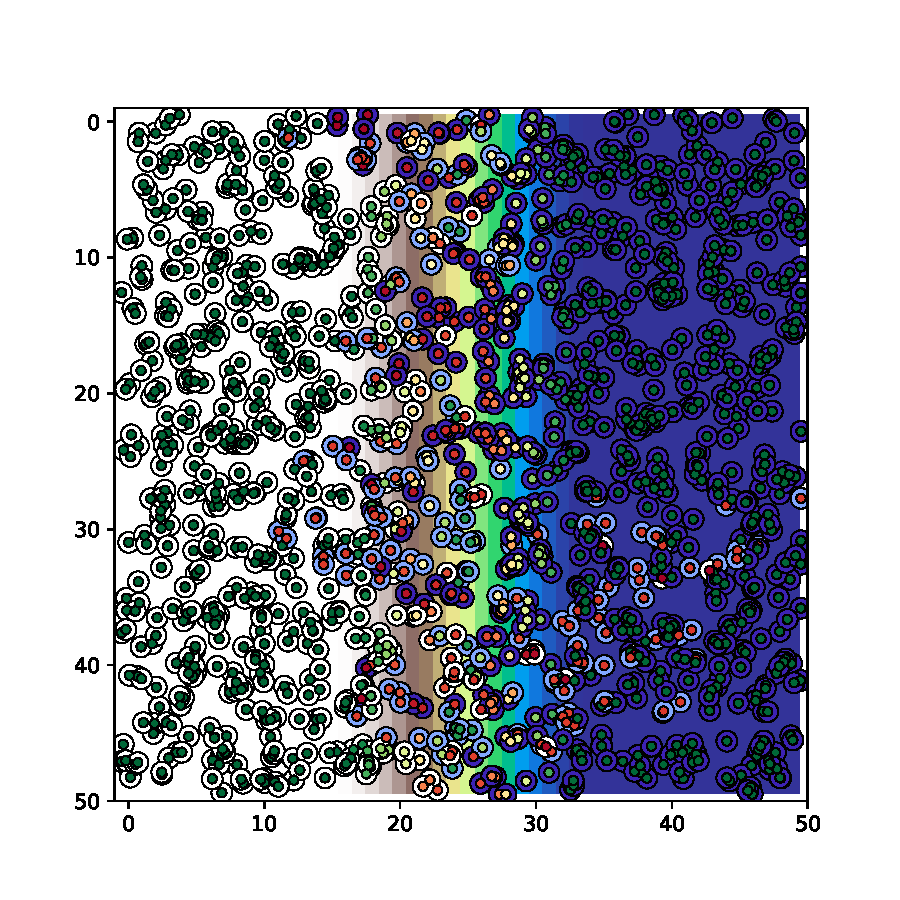
\includegraphics[width=175mm]{./img/final/CLINE_pop_plot.pdf}
        \caption{Cline test: Map of the final population
                 on top of the selective landscape layer,
                 with individuals colored by phenotype (outer circles)
                 and fitness (inner circles), as in Figure~\ref{fig:div_pop}.
                 (Plot was produced by the Geonomics method
                 \texttt{model.plot\_fitness}.)}
        \label{fig:cline_pop}
\end{figure}



\begin{figure}[!p]
        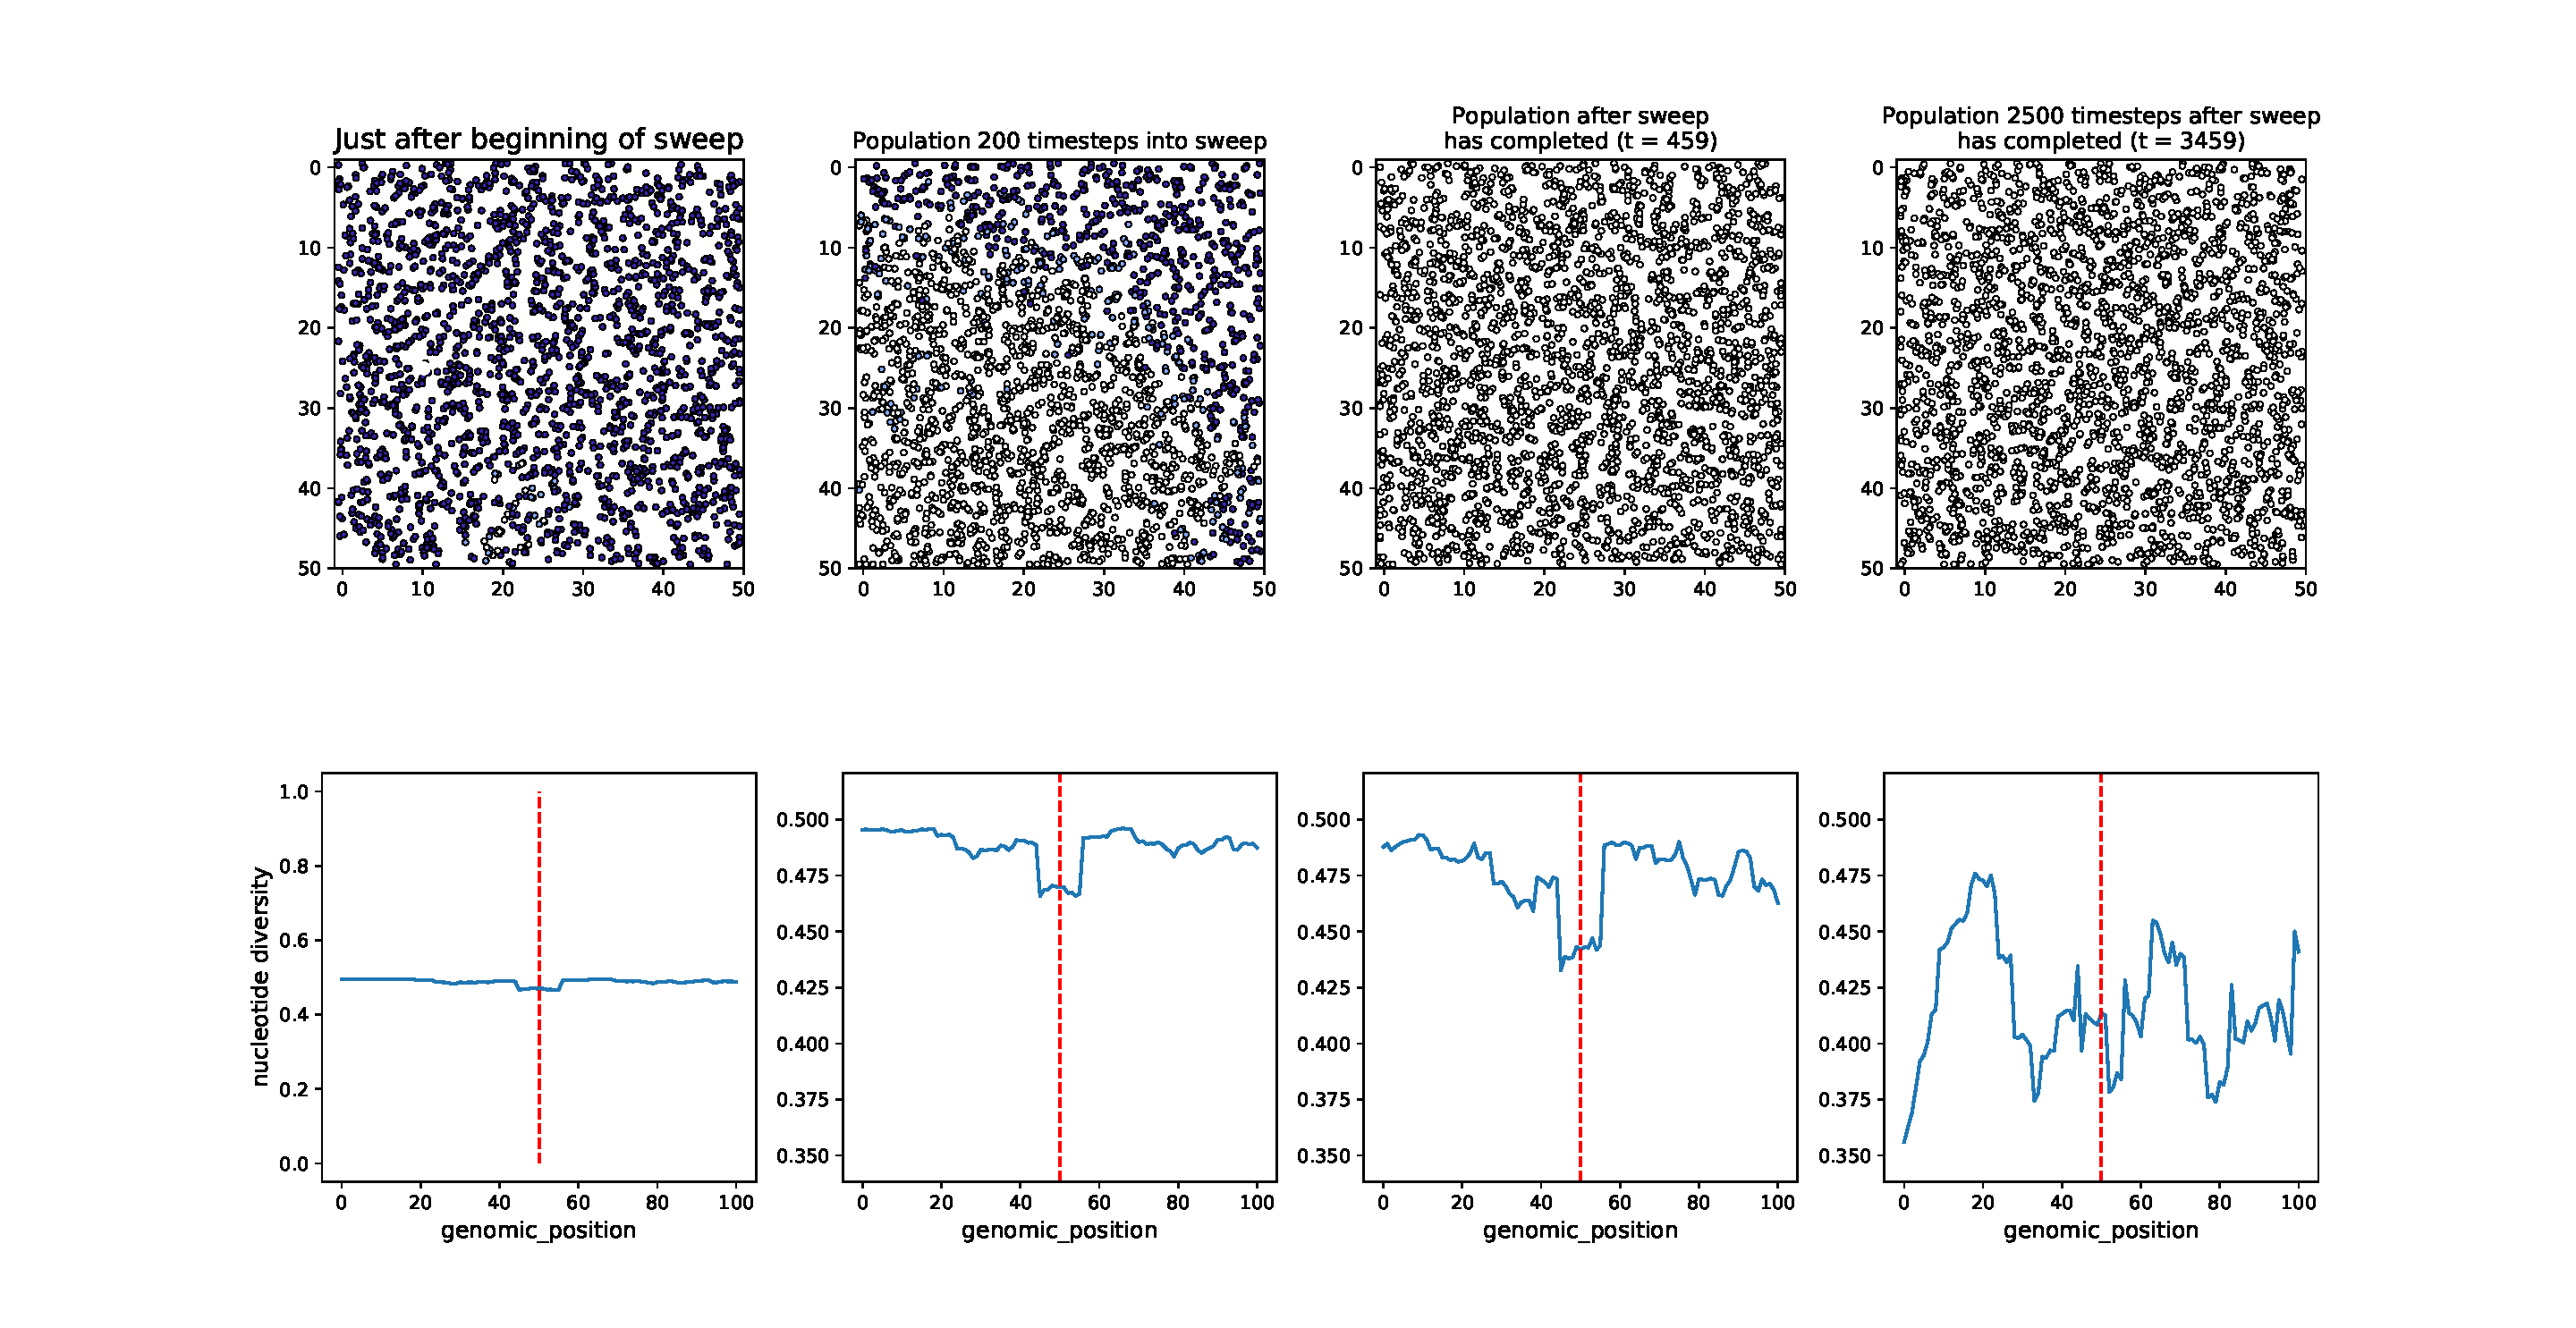
\includegraphics[width=175mm]{./img/final/SWEEP_pop_and_nuc_div.pdf}
        \caption{Selective sweep test: Maps of population (top row;
                 colored by phenotype, as in Figure~\ref{fig:div_pop})
                 and genome-wide nucleotide diversity
                 (bottom row; calculated in $\leq$~11-locus windows)
                 at various points in time during the model run
                 (from left to right: timestep 0, 
                 timestep 200, just after completion of the sweep,
                 and 2500 timesteps after completion of the sweep).
                 (Top-row plots were produced by the Geonomics method
                 \texttt{model.plot\_phenotype}.)}
       \label{fig:sweep_pop_and_nuc_div}
\end{figure}



\begin{figure}[!p]
        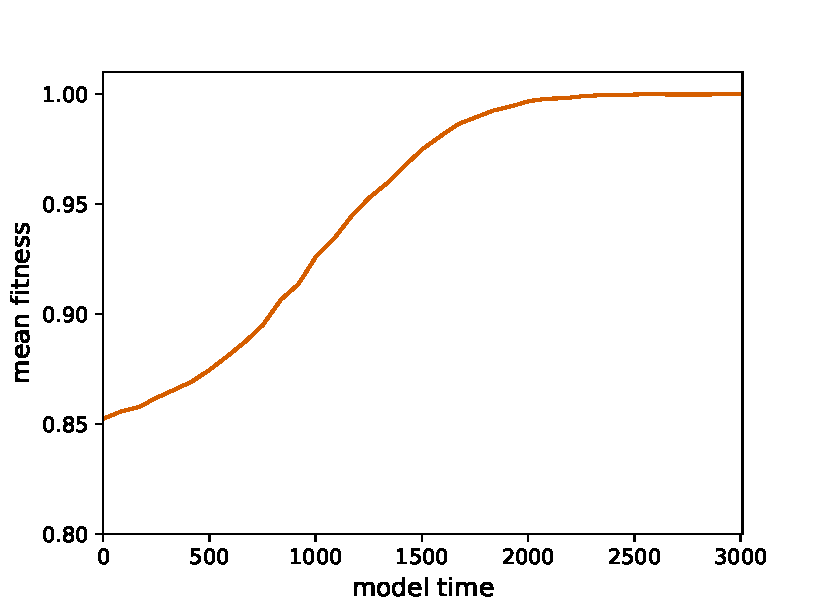
\includegraphics[width=150mm]{./img/final/SWEEP_mean_fit.pdf}
        \caption{Selective sweep test: Mean fitness of the entire
                 population, over the full run of the model
                 depicted in Figure~\ref{fig:cline_pop}}
        \label{fig:sweep_fit}
\end{figure}


\end{document}
